\documentclass[preprint2]{aastex62}
\graphicspath{ {./figs/} }
\usepackage{xspace, url}
%% \documentclass[twocolumn,linenumbers,trackchanges]{aastex61}
%%
\renewcommand{\figureautorefname}{Fig.}
\renewcommand{\sectionautorefname}{\S}
\renewcommand{\subsectionautorefname}{\S}
\renewcommand{\subsubsectionautorefname}{\S}
\renewcommand{\equationautorefname}{Eq.}
\renewcommand{\tableautorefname}{Table}
%% 
\newcommand{\Fig}[1]{\autoref{fig:#1}}
\newcommand{\Sec}[1]{\autoref{sec:#1}}
\newcommand{\Tab}[1]{\autoref{tab:#1}}
\newcommand{\Eq}[1]{\autoref{eq:#1}}
%% 
\newcommand{\z}[1]{$z \sim {#1}$}
\newcommand\vs{\ensuremath{\mathrm{vs.}}\xspace}
\newcommand{\FSPS}{{\sc FSPS}\xspace}
\newcommand{\pFSPS}{{\tt \textbf{python-fsps}}\xspace}
\newcommand{\CloudyFSPS}{{\tt \textbf{CloudyFSPS}}\xspace}
\newcommand{\Mappings}{{\sc Mappings-III}\xspace}
\newcommand{\Pegase}{\textsc{P{\'e}gase}\xspace}
\newcommand{\SB}{\textsc{Starburst-99}\xspace}
\newcommand{\Cloudy}{\textsc{Cloudy}\xspace}
\newcommand{\hii}{H\,{\sc ii}\xspace}
\newcommand{\nii}{[N\,{\sc ii}]\xspace}
\newcommand{\sii}{[S\,{\sc ii}]\xspace}
\newcommand{\oiii}{[O\,{\sc iii}]\xspace}
\newcommand{\oii}{[O\,{\sc ii}]\xspace}
\newcommand{\oi}{[O\,{\sc i}]\xspace}
\newcommand\Lsun{\ensuremath{\,\mathrm{L_{\sun}}}\xspace}
\newcommand\Msun{\ensuremath{\,\mathrm{M_{\sun}}}\xspace}
\newcommand{\ha}{\ensuremath{\mathrm{H\alpha}}\xspace}
\newcommand{\hb}{\ensuremath{\mathrm{H\beta}}\xspace}
\newcommand{\logten}{\ensuremath{\log_{10}}}
\newcommand{\logz}{\ensuremath{\logten \mathrm{Z}/\mathrm{Z}_{\sun}}\xspace}
\newcommand{\logZeq}[1]{\ensuremath{\logten \mathrm{Z}/\mathrm{Z}_{\sun} = #1}}
\newcommand{\ang}{\ensuremath{\mbox{\AA}}\xspace}
\newcommand{\logQ}[1]{\ensuremath{\logten Q_{#1}}}
\newcommand{\QH}{\ensuremath{Q_{\mathrm{H}}}\xspace}
\newcommand{\QHe}{\ensuremath{Q_{\mathrm{He}}}\xspace}
\newcommand{\QHat}{\ensuremath{\hat{Q}_{\mathrm{H}}}\xspace}
\newcommand{\QHehat}{\ensuremath{\hat{Q}_{\mathrm{He}}}\xspace}
\newcommand{\U}{\ensuremath{\mathcal{U}_{0}}\xspace}
\newcommand{\logU}{\ensuremath{\logten \mathcal{U}_0}}
\newcommand{\logUeq}[1]{\ensuremath{\logten \mathcal{U}_0 = #1}}
\newcommand{\kms}{\ensuremath{\;\mathrm{km}\;\mathrm{s}^{-1}}\xspace}
\newcommand{\Myr}{$\,$Myr\xspace}
\newcommand{\Gyr}{$\,$Gyr\xspace}
\newcommand{\Av}{\ensuremath{A_{\mathrm{V}}}\xspace}
\newcommand{\dAv}{\ensuremath{\mathrm{d}A_{\mathrm{V}}}\xspace}
\newcommand{\dmod}{\ensuremath{(M - m)_0}\xspace}
%%
\newcommand{\vdag}{(v)^\dagger}
\newcommand\aastex{AAS\TeX}
\newcommand\latex{La\TeX}
%%%%%%%%%%%%%%%%%%%%%%%%%%%%%%%%%%%%%%%%%%%%%%%%%%%%%%%%%%%%%%%%%%%%%%%%%%%%%%%%
%%
%\received{July 1, 2016}
\revised{\today}
%\accepted{\today}
%\submitjournal{ApJ}
%%
\shorttitle{Calibrating SPS models with resolved stellar populations}
\shortauthors{Byler et al.}
%%
%%%%%%%%%%%%%%%%%%%%%%%%%%%%%%%%%%%%%%%%%%%%%%%%%%%%%%%%%%%%%%%%%%%%%%%%%%%%%%%%
\begin{document}
\title{Using resolved stellar populations to improve the recovery of star formation histories from galaxy spectra}
%%%%%%%%%%%%%%%%%%%%%%%%%%%%%%%%%%%%%%%%%%%%%%%%%%%%%%%%%%%%%%%%%%%%%%%%%%%%%%%%
%%
\author[0000-0002-7392-3637]{Nell Byler}
\affil{Research School for Astronomy and Astrophysics, Australian National University, Mount Stromlo Observatory, Cotter Road, Weston Creek, ACT 2611, AUSTRALIA}
%% 
\author[0000-0003-4122-7749]{O. Grace Telford}
\affil{Department of Astronomy, University of Washington, Box 351580, Seattle, WA 98195, USA}
%% 
\author[0000-0002-1264-2006]{Julianne J. Dalcanton}
\affil{Department of Astronomy, University of Washington, Box 351580, Seattle, WA 98195, USA}
%%
\author[0000-0002-6442-6030]{Daniel R. Weisz}
\affil{Department of Astronomy and Theoretical Astrophysics, University of California Berkeley, Berkeley, CA 94720, USA}
%%
\author[0000-0002-9280-7594]{Benjamin D. Johnson}
\affil{Department of Astronomy, Harvard University, Cambridge, MA, USA}
%%
\author[0000-0002-1590-8551]{Charlie Conroy}
\affil{Department of Astronomy, Harvard University, Cambridge, MA, USA}
%%
\author[0000-0002-7502-0597]{Benjamin F. Williams}
\affil{Department of Astronomy, University of Washington, Box 351580, Seattle, WA 98195, USA}
%%
%%%%%%%%%%%%%%%%%%%%%%%%%%%%%%%%%%%%%%%%%%%%%%%%%%%%%%%%%%%%%%%%%%%%%%%%%%%%%%%%
\begin{abstract}

Nearby galaxies provide a unique opportunity to evaluate the accuracy of recovering the history of star formation from fitting integrated light spectra. Within ${\sim}4\,$Mpc, galaxies are close enough to be resolved into individual stars, but distant enough that their angular sizes are comparable current integral field unit (IFU) sizes. In this work we compare IFU spectroscopy from a MaNGA ancillary program to spectra inferred from star formation histories (SFH) derived from color-magnitude diagrams (CMDs) within nearby dwarf galaxy NGC 4163. Using the CMD-based SFH as input to a stellar population synthesis (SPS) code, we show that the resultant model spectrum is in good overall agreement with the aperture-matched, summed spectrum. We discuss strengths and weaknesses of CMD and integrated light analyses, including the ability of CMDs to inform issues such as differential extinction, stochastic sampling of the IMF, and the presence of ancient populations, each of which can be challenging to discern from spectroscopy alone. The findings of this work provide a useful empirical test for consistent measurement of SFHs in the nearby and distant Universe, and for the validity of widely used SPS models.

\end{abstract}
%\keywords{Galaxies --- galaxies: emission lines --- galaxies: abundances --- galaxies: ISM}
%%%%%%%%%%%%%%%%%%%%%%%%%%%%%%%%%%%%%%%%%%%%%%%%%%%%%%%%%%%%%%%%%%%%%%%%%%%%%%%%
\section{Introduction} \label{sec:intro}

The use of Stellar Population Synthesis (SPS) models is ubiquitous in extragalactic astronomy. In these models, one adds together ``simple stellar populations’’ or SSPs (e.g., stars of a single age and chemical composition), weighted by a star formation history (SFH; e.g., the mass in stars formed at each age) to produce a galaxy spectrum. These synthetic spectra are routinely used to translate observed galaxy flux into meaningful physical properties like stellar mass, star formation rate (SFR), age, and metallicity \citep[see reviews in][]{Walcher+2011, Conroy+2013}.

In principle, deriving these critical astrophysical quantities from a given galaxy spectrum is a straight-forward minimization problem to identify the best-fit model. In practice, however, the degeneracies are significant, and one typically needs to adopt a host of simplifying assumptions about dust geometry, chemical enrichment, and the SFH. As such, SPS models provide a profound physical intuition for understanding galaxy spectra when used in one direction (i.e., to predict how a given set of parameters will affect the emergent spectrum). However, it is unclear whether or not the derived properties accurately represent the true galaxy properties, when used in the other direction (i.e., to infer physical parameters from observed spectra). 

The fundamental difficulty in using SPS models to derive physical properties from galaxies is that the youngest populations dominate the integrated light and conceal older populations, yielding uncertain estimates of stellar mass and age. Likewise, degeneracies between SFH, dust attenuation, and metallicity make it difficult to extract both past and present SFRs.

To break the many degeneracies inherent in SPS modeling, SED fitting codes are typically forced to assume a simple functional form for the SFH. Unfortunately, any deviation from the assumed SFH parameterization introduces biases in the derived galaxy properties \citep[e.g., ][]{Lee+2009, Maraston+2010, Pforr+2012}.  Further complexity is introduced by the choice of fit parameters and priors, and different SED fitting codes often produce different solutions for key parameters like stellar mass and SFR \citep[e.g, ][]{Santini+2015, Goddard+2017, Li+2017, Ge+2018}. Without outside calibration data, it is impossible to know which fitting strategy produces the most reliable results.

One example of calibration data is the \citet{Brown+2014} spectral atlas, which includes low-resolution optical spectra aperture-matched to photometry for 129 nearby galaxies. \citet{Leja+2017} fit the broadband UV-IR photometry for each galaxy and compared model predictions to the aperture-matched spectroscopy to test the reliability of SFR and SFH estimates from SED-fitting. \citeauthor{Leja+2017} found that \ha luminosities predicted from fits to the photometry were in good agreement with the observed luminosities across a range of galaxy types and stellar masses, a strong verification of the model SFRs. The authors also found good agreement between model predicted SFH indicators ($D4000$, H$\delta$ absorption). \citeauthor{Leja+2017} found that the broadband photometry could not uniquely constrain changes in SFH on timescales shorter than $\sim100$\Myr. Additionally, broadband photometry does not provide tight constraints on stellar populations older than $\sim1$\Gyr, and the ability to accurately recover the SFH ultimately decreases with lookback time.

Nearby galaxies provide a unique opportunity to assess the accuracy and bias in the ages and SFRs recovered from integrated light techniques. These galaxies are close enough to be resolved into individual stars, enabling the construction of color-magnitude diagrams (CMDs). Star formation imprints a clear, historical record in the structure and relative strengths of the main sequence, helium burning sequences, red giant branch, and horizontal branch of a CMD. These prominent CMD features can be modelled to extract quantitative SFHs from resolved stellar populations. The well-developed method of synthetic CMD fitting constrains the actual history of star formation with more absolute and temporal precision than is possible with spectral fitting \citep[see \citet{Tolstoy+2009} and references therein; also ][]{Weisz+2011}.

We can directly compare the ``ground truth'' SFH from resolved stars with the SFH determined from integrated light using galaxies that can be targeted with both integral field spectroscopy (IFS) and the Hubble Space Telescope (HST). Unfortunately, the observational requirements for this comparison are restrictive, and there are a limited number of galaxies that are well-suited for the task. First, the galaxy must be close enough to be resolved into individual stars with HST ($\lesssim4$\,Mpc). Second, the galaxy must also be distant enough such that the angular extent is well-matched to the field of view of typical integral field unit (IFU) instruments (${\sim}0.1-2$').

The nearby dwarf galaxy NGC 4163 fulfills both of these requirements. Not only is it well matched to both HST and IFU instruments ($D \sim 3$\,Mpc, $r_{\mathrm{h}} \sim 0.5$'), but its low dust content ($\Av \sim 0.06$) ensures a clean test of SFH-inference, relatively uncomplicated by dust-metallicity degeneracies. This galaxy has deep multi-band imaging from HST, analyzed as a part of the ACS Nearby Galaxy Survey Treasury \citep[ANGST;][]{Dalcanton+2009, Dalcanton+2012}. We subsequently observed NGC 4163 with an IFU from the Mapping Nearby Galaxies at APO \citep[MaNGA;][]{Bundy+2015} survey in Spring 2014 as part of an ancillary program.

Our analysis proceeds along two paths: First, we use the CMD-based SFH as input to an SPS code and compare the resultant model spectrum with the aperture-matched, summed spectrum from MaNGA. Second, we use a spectral fitting code on the summed MaNGA spectrum and compare the derived galaxy properties to those derived from CMD-fitting methods. Both analyses provide a useful empirical test for the consistent measurements of SFHs, and for the validity of widely used SPS models. 

A comparison of the parameters derived with SED fitting and CMD-fitting has been done in the context of single-aged, single-abundance populations like star clusters \citep[e.g., ][]{Gibson+1999, Beasley+2002, Delgado+2010, Thomas+2011, Barber+2014, Kuncarayakti+2016, Usher+2017}. For more complex stellar populations, \citet{Ruiz-Lara+2015} and \citet{Ruiz-Lara+2018} compare the SFH recovered from CMD-fitting with the SFH recovered from spectral fitting in subregions of the Large Magellenic Cloud (LMC) and Leo A. In \citet{Ruiz-Lara+2015}, the authors compare the CMD-recovered SFH with SFHs derived with different spectral fitting codes to gain insight into the most successful parametrizations. The authors found the best agreement in SFH using fitting techniques that preferred smooth SFH solutions, as implemented in STECMAP \citep{Ocvirk+2006}. To improve constraints from CMD-fitting, \citet{Ruiz-Lara+2018} extended the original study to Leo A, an object where photometry reaches below the oldest main sequence turn-off.

Both studies were able to match the general shape of the CMD-derived SFH, but with discrepancies in the derived age-metallicity relationships (AMR). We note that Leo A also has a fairly atypical SFH, with a small old stellar population (just $\sim10$\% of its total stellar mass was formed in the first 6\Gyr of SF). Moreover, both the LMC and Leo A are very young systems, with $\sim50$\% of their total stellar mass formed in the last 2-4\Gyr. These comparisons likely represent the best-case scenario for SFHs recovered from integrated light, where young stars vastly outshine the older stellar population. In this work, we build upon the \citet{Ruiz-Lara+2015} and \citet{Ruiz-Lara+2018} studies, and compare SFH determinations in an object with recent star formation and a substantial old stellar population. \textbf{XXX: do i mention that other differences? (1) Different CMD-fitting code, (2) Higher resolution spectra: FWHM$\sim2-3$\ang (SDSS) compared to FWHM$\sim10$\ang (Ruiz-Lara+2018), (3) better wavelength coverage (4000-5000\ang for Ruis-Lara+2018), (4) Fiber bundle instead of slit.}

In addition to assessing the SFH-recovery of spectral fitting codes, we extend the \citet{Ruiz-Lara+2018} to new territory by using the CMD-derived SFH as input to an SPS code and comparing the model and observed spectrum, which tests the SPS model ingredients. This was first done for complex stellar populations in \citet{Johnson+2013}, where the authors combined the CMD-inferred SFH with SPS models to predict the UV through NIR broadband SED of $\sim50$ galaxies from the ANGST survey, and compared with the observed SEDs. \citet{Johnson+2013} found good agreement between predicted and observed SEDs at optical wavelengths, but had to adopt a differential extinction model in order to match the UV filters. The largest discrepancies were at NIR wavelengths, likely the result of the specific model treatment of uncertain phases of evolved stellar evolution (i.e., thermally pulsing asymptotic giant branch stars). Here, we make a similar comparison, but with a detailed comparison of optical spectral features.

The paper is structured as follows. We describe the data in \S\ref{sec:data}, covering the MaNGA observations and data reduction techniques in \S\ref{sec:data:manga}, and the HST observations in \S\ref{sec:data:hst}. We outline our analysis techniques in \S\ref{sec:methods}, including the CMD-fitting of the resolved stellar population using MATCH (\S\ref{sec:methods:match}), and synthesizing a model spectrum from CMD-inferred properties (\S\ref{sec:methods:fsps}). In \S\ref{sec:results}, we compare the aperture-matched summed MaNGA spectrum to the model spectrum. We discuss uncertainties associated with differential extinction, stellar models, IMF, and age-metallicity relations in \S\ref{sec:discussion}. In \S\ref{sec:conclusions} we summarize our conclusions.

\section{Data}\label{sec:data}

NGC 4163 is a nearby dwarf galaxy with low-metallicity ([M/H]$\sim -1$) and recent star formation\citep{ Kennicutt+2008, Lee+2009}. The global SFH of NGC 4163 shows sustained star formation over the last 300\Myr, with a decline in SFR at most recent times \citep{McQuinn+2010}. We summarize the observed properties of NGC 4163 in Table~\ref{tab1}.

%\footnotesize
%\begin{landscape}
\begin{deluxetable*}{ccccccc}
\tablecolumns{7}
\tabletypesize{\scriptsize}
\tablewidth{0pt}
\tablecaption{NGC\,4163 Properties}
\tablehead{
    \colhead{$M_{B}$} & % absolute blue magnitude Karachentsev et al. 2004
    \colhead{D} & % TRGB distance (Dalcanton et al. 2009)
    \colhead{$A_{V}$} & %foreground extinction (Schlegel et al. 1998)
    \colhead{T} & % morphological T Type (de Vaucouleurs et al. 1991; Karachentsev et al. 2004)
    \colhead{$\log_{10}(\mathrm{SFR}_{\mathrm{UV}})$} &
    \colhead{ $ 12 + \log_{10} ( \mathrm{O} / \mathrm{H} ) $ } & % 12 + log(O/H) (Berg+2012)
    \colhead{ $ \log_{10} ( \mathrm{N} / \mathrm{O} ) $ } \\ % log(N/O) (Berg+2012)
        \colhead{} & %M_B
        \colhead{(Mpc)} & %Distance
        \colhead{} & % Av
        \colhead{} & %T
        \colhead{$\mathrm{M}_{\odot}\cdot \mathrm{yr}^{-1}$} & % SFR
        \colhead{dex} & %O/H
        \colhead{dex} \\ % N/O
            \colhead{(1)} & % M_B
            \colhead{(2)} & % Dist
            \colhead{(3)} & % Av
            \colhead{(4)} & % T
            \colhead{(5)} & % SFR
            \colhead{(6)} & % OH
            \colhead{(7)}   % NO
      }
\startdata
-13.76 & 2.88$\pm$0.04 & 0.055 & 10 & -2.34 & $7.56 \pm 0.04$ & $-1.49 \pm 0.06$ \\
% M_B  & dist          & A_v   & T  & 12+logOH        & log(N/O)
\enddata
\tablecomments{(1) Absolute Blue Magnitude \citep{Karachentsev+2004}; (2) TRGB Distance \citep{Dalcanton+2009}; (3) Foreground extinction \citep{Schlegel+1998}; (4) Morphological T-Type \citep{Karachentsev+2004}; (5) log SFR from \citet{Lee+2009} calculated from integrated GALEX FUV magnitude with \citet{Kennicutt+1998}; (6) direct-temperature oxygen abundance \citep{Berg+2012}; (7) Nitrogen to oxygen ratio \citep{Berg+2012}.}
\label{tab1}
\end{deluxetable*}

% <SFR> lifetime 8.92 +1.44 −1.38 * 10^-3 Msun/yr (Weisz+2011) >> log(SFR) = -2.1
% 2.88 +/- 0.04 Mpc from TRGB, Dalcanton 2009 // Av = 0.06 and 27.29
% E(B-V) = 0.017; Schlafly & Finkbeiner (2011)
% m-M = 27.38 + 0.03, -0.02 (F814W TRGB distance; Wu 2014)
% no He I emission or Ne III (Berg+2012)
% 12+log(O/H) = 7.56 ± 0.14 (Berg+2012)
% log(N/O) = −1.49 ± 0.06 (Berg+2012)
% PARSEC: -1.0
% youngest age in parsec is 3.5 Myr (Rosenfield)
% Lee+2009 ratio = -0.21 >> log(SFR_Ha) = -2.55
% SFR(M yr−1) = 7.9 × 10−42 L(Hα) (erg s−1) K98
%\footnotesize
%\begin{landscape}
\begin{deluxetable*}{ccccccccc}
\tablecolumns{9}
\tabletypesize{\scriptsize}
\tablewidth{0pt}
\tablecaption{MATCH parameters}
\tablehead{
    \colhead{$A_{V}$} & %foreground extinction (Schlegel et al. 1998)
    \colhead{$(m-M)_0$} & % distance modulus
    \colhead{$M_{F814W}$ 50\%} &
    \colhead{$M_{F814W}$ 50\%} \\
        \colhead{} & % Av
        \colhead{} & % dmod
        \colhead{Completeness} &
        \colhead{Completeness} \\
            \colhead{(3)} & %Av
            \colhead{(4)} & %dmod
            \colhead{(8)} &
            \colhead{(9)}
      }
\startdata
0.055 & $27.38\pm0.03$ & -0.04 & -0.04\\
% A_v   & dmod         & comp  & comp
\enddata
\tablecomments{(1) Foreground extinction \citep{Schlegel+1998}; (2) distance modulus, F814W Wu+2014; (3)  50\% completeness limit ($M_{F606W}$); (4)  50\% completeness limit ($M_{F814W}$).}
\label{tab2}
\end{deluxetable*}

\subsection{MaNGA observations of NGC 4163}\label{sec:data:manga}

MaNGA, part of SDSS IV \citep{Blanton+2017}, is an IFU survey with the goal to obtain spatially resolved spectroscopy for statistically representative sample of 10,000 galaxies in the redshift range $0.01 < z < 0.15$. MaNGA uses hexagonal fiber bundles paired with the dual beam BOSS spectrographs, which cover the wavelength range from 3600\ang to 10,300\ang with a spectral resolution $R\sim2000$ \citep{Smee+2013}.

The MaNGA data used in this work were reduced using version {\tt v2\_0\_1} of the MaNGA data reduction pipeline \citep{Law+2016} for MaNGA product launch 5 (MPL5) and part of the SDSS data release 13 \citep{Albareti+2017}.

NGC 4163 was observed as an ancillary target in Spring 2014. We used a 127-fiber IFU following the standard MaNGA procedures, which consist of three 15-minute exposures at each of the 3-point dither positions, for a total integration time of 2 hours and 15 minutes. The standard observing strategy is described in detail in \citet{Yan+2016}, see also \citet{Law+2015}.

In Fig.~\ref{fig:FOV}, we show an image of NGC 4163 in the F606W filter, with the approximate location of the MaNGA footprint shown with the black hexagon. The spatial distribution of luminous main sequence stars is shown with blue circular markers, revealing regions of vigorous star formation and more quiescent regions. At 3\,Mpc, NGC 4163 is much closer than typical MaNGA galaxies, and the IFU footprint only covers a fraction of the total galaxy. For reference, the 127-fiber IFU has a diameter of $0.54$', while the the half-light radius for NGC 4163 is 0.45'$\pm0.05$ \citep{McConnachie+2012}. In contrast, the galaxy is well covered by the HST observations, where the field of view of the ACS camera is 2' on a side.

Within the footprint of the MaNGA observations, there are approximately 7,000 stars resolved with HST. For statistical robustness, the CMD-fitting process requires at least ${\sim}10^3$ stars. We therefore use the entire area covered by the MaNGA observations in our aperture-matched analysis. 

The individual fiber spectra from all exposures are combined into a single data cube using the astrometric solution (derived for each fiber based on the IFU bundle metrology) and a nearest neighbor sampling algorithm. The data cube has linear wavelength sampling from from 3622\ang to 10353\ang with 6732 spectral elements and 0.5'' spatial pixels (spaxels).
%%%
%-------------------------------------------------------
\begin{deluxetable}{cc}
\tablecolumns{2}
\tabletypesize{\scriptsize}
\tablewidth{0pt}
\tablecaption{Coordinates of polygon used for aperture-matching}
\tablehead{
    \colhead{RA (J2000)} &
    \colhead{Dec (J2000)}
      }
\startdata
183.0429 & 36.1725\\
183.0422 & 36.1730\\
183.0397 & 36.1733\\
183.0371 & 36.1734\\
183.0358 & 36.1729\\
183.0355 & 36.1720\\
183.0347 & 36.1717\\
183.0343 & 36.1712\\
183.0333 & 36.1698\\
183.0332 & 36.1685\\
183.0342 & 36.1675\\
183.0342 & 36.1671\\
183.0346 & 36.1670\\
183.0345 & 36.1666\\
183.0351 & 36.1659\\
183.0353 & 36.1653\\
183.0364 & 36.1647\\
183.0377 & 36.1648\\
183.0381 & 36.1645\\
183.0383 & 36.1648\\
183.0411 & 36.1645\\
183.0417 & 36.1647\\
183.0427 & 36.1657\\
183.0432 & 36.1665\\
183.0449 & 36.1683\\
183.0449 & 36.1691\\
183.0440 & 36.1704\\
183.0437 & 36.1709
\enddata
\tablecomments{None}
\label{tabel3}
\end{deluxetable}

%-------------------------------------------------------

To create an identical spatial region for the aperture-matched comparison, we manually select coordinates to construct a hexagonal polygon, which is then used to spatially select both the MaNGA spaxels and the resolved stellar population. The coordinates of the polygon are given in Table~\ref{tabel3}, shown as the black outline in Fig.~\ref{fig:FOV}.

The hexagonal region covers $N=3266$ spaxels, with S/N ranging from 5-100. We use the MaNGA pixel mask to remove spaxels flagged as ``unacceptable'' for science use ($N=200$, roughly 6\% of the 3266 spaxels in the aperture matched region). These masked spaxels are located at the outer edges of the IFU, and contribute less than $5-7$\% of the total flux. The total summed integrated spectrum includes $N=3066$ spaxels and has S/N $\sim800$ at $\lambda=5500\ang$. 
% 3528 / 5776 spaxels are "covered" by the hex
% 448 of these are further flagged as "do not use". These are all at the outer edges of the IFU, and contribute 5-7% of the total flux.
% in hex region: 3266 / 5776; 200 are further flagged as "do not use".

\textbf{XXX JD asks: total area and completeness / do we really capture all the flux? Don't want referee asking about filling factors in the IFU and PSF losses from the edges. Nell: I added in some text referencing the flux contribution of "bad" spaxels that I remove, but I do not remove spaxels flagged as ``low-coverage'', $\lesssim 10\%$ of total flux.}

%-------------------------------------------------------
% Figure 1: F606W image with footprint
%-------------------------------------------------------
\begin{figure*}
  \begin{center}
    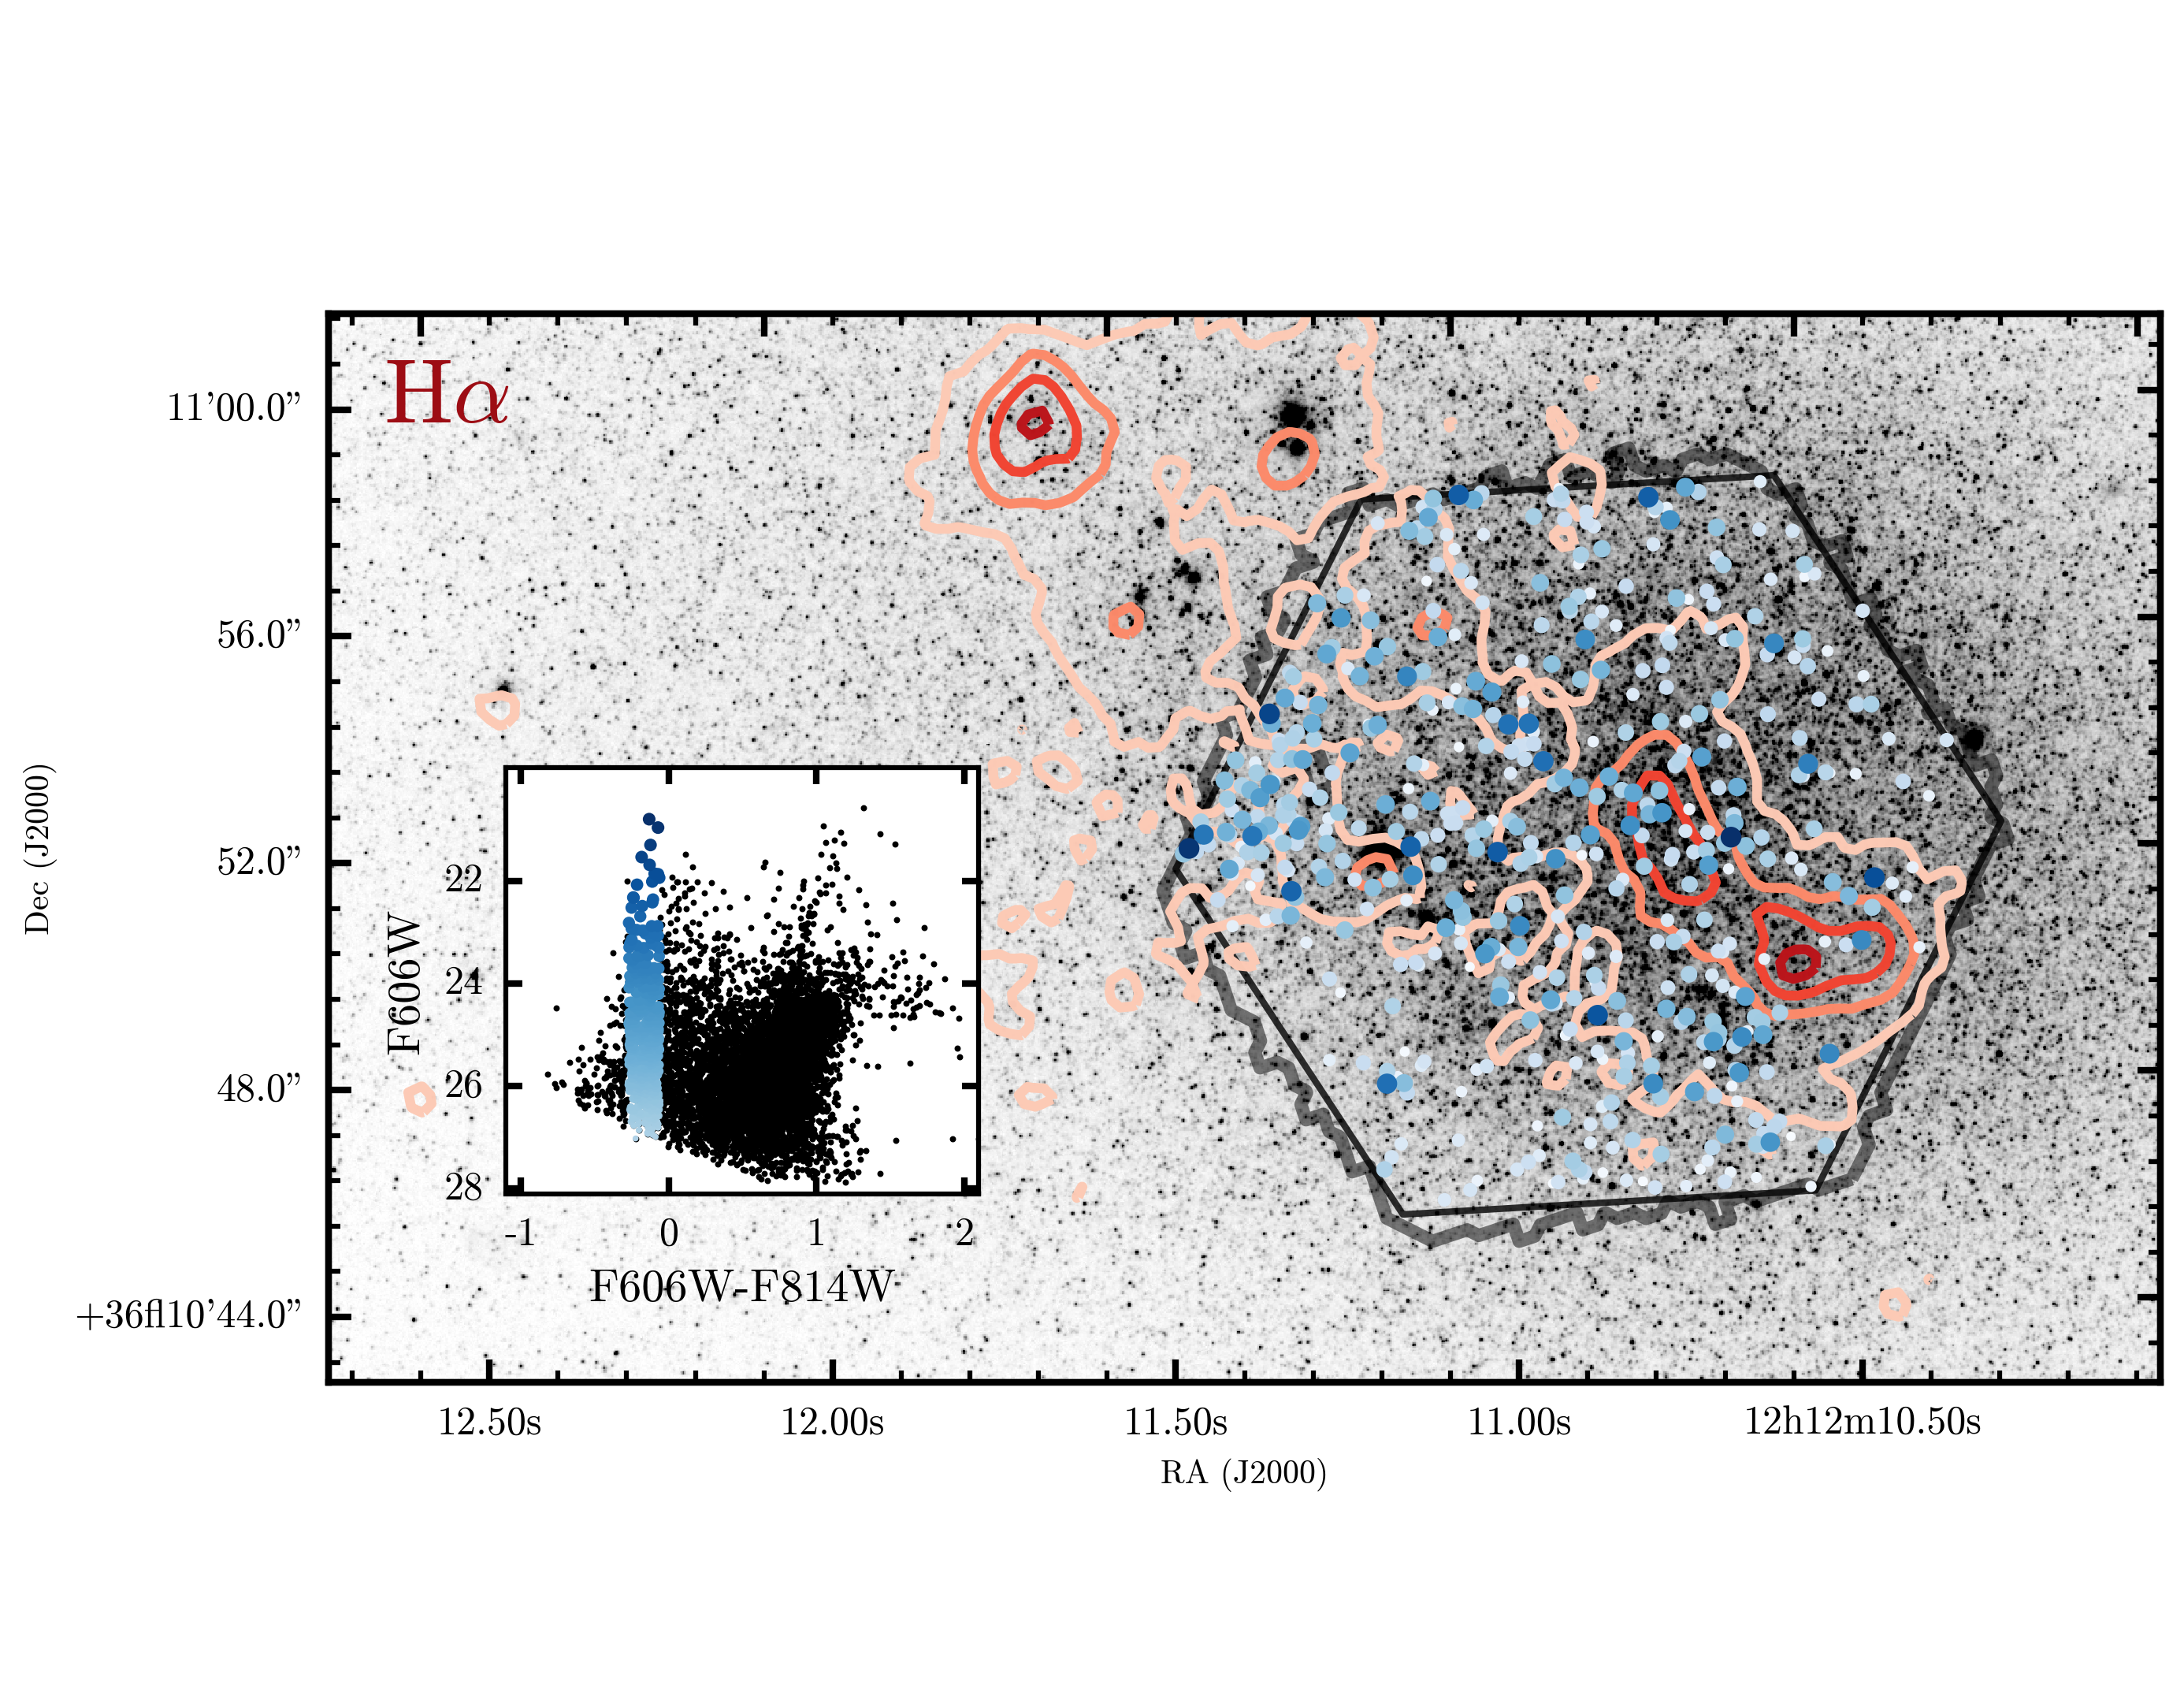
\includegraphics[width=\linewidth]{figs/f1.png}
    \caption{We show the F606W image of NGC 4163, with the footprint of the MaNGA observations approximated with the black hexagon. \ha contours from the LEGAS survey are shown in red (\textbf{XXX cite}), with the strongest \ha emission shown in the darkest red lines. In the bottom left corner of the figure, we show an inset colour-magnitude diagram, F606W-F814W \vs F606W, with main sequence stars highlighted in blue, where darker blue points represent more luminous main sequence stars. The spatial location of the selected main sequence stars is also shown on the F606W image. Young, hot stars are located throughout the MaNGA observation, with some spatial clustering near known OB associations.}
    \label{fig:FOV}
  \end{center}
\end{figure*}
% actual boundary is weirder though. Do you have an exposure time map for MaNGA showing actual depth accross field after dithering? Hard to see faint MS stars, add MaNGA obs PSF and spaxel size. Leaking edges?
%-------------------------------------------------------

\subsection{HST observations of NGC 4163}\label{sec:data:hst}

NGC 4163 has multi-band archival imaging from HST, analyzed as a part of the ACS Nearby Galaxy Survey Treasury \citep[ANGST;][]{Dalcanton+2009, Dalcanton+2012}. Full details of the survey and photometry can be found in \citet{Dalcanton+2009}.

We use optical photometry (F475W and F606W filters) from the ``{\tt .gst}'' catalogs, which only include stars with the highest quality photometry. The ``{\tt .gst}'' catalogs were compiled following procedures developed by \citet{Dolphin+2000} as described in \citet{Dalcanton+2012}. The stars in the ``{\tt .gst}'' catalog have S/N$ > 4$ in both filters and pass stringent goodness-of-fit cuts. These cuts leave stars with the highest quality photometry but with higher incompleteness in more crowded regions. We then select those stars that fall within the boundary of the MaNGA IFU observation boundaries to create a single catalog of aperture-matched stars.

\textbf{XXX Actually, Dan re-ran the photometry around 7/1/16: }\emph{``The photometry is of the entire ACS field, while the fake stars are just for a region around the MANGA footprint. These are only roughly gst files — I did this by hand and couldn't remember the exact data naming scheme.  It should be self-explanatory, but you'll have to check to make sure you're grabbing the correct columns. I've also already applied quality cuts to the photometry and fake stars.  So all you have to do is grab the data, cut out the RA and DEC region of interest, and run it through MATCH — you don't need to apply any photometric quality cuts.''} \textbf{@Dan: I'm assuming ``roughly gst'' means the files may not have correct naming convention or proper columns, but quality cuts are still those described in Dalcanton+2012? Are there any important details about the new photometry I should include?}

In Fig.~\ref{fig:cmd}, we show two CMDs for NGC 4163. The CMD shown in the left panel includes photometry from the full ACS field of view (${\sim}74,000$ stars), while the right panel shows the photometry extracted from the region mapped to the MaNGA observations (${\sim}7,000$ stars). The arrow shows the direction of 1 magnitude of extinction, and the black and blue lines show the 50\% and 80\% completeness limits, respectively. \textbf{XXX: completeness limits not yet shown}

The full-field CMD (left panel of Fig.~\ref{fig:cmd}) shows a well-defined red giant branch (RGB), a well-populated red clump (RC) and main sequence (MS). In the aperture-matched CMD (right panel of Fig.~\ref{fig:cmd}), the MS and RGB are also evident. However, the photometry in the aperture-matched region is significantly shallower than the photometry from the full field, due to higher crowding in the central region of the galaxy. Crowding in regions with high stellar density can strongly affect the photometry, since fewer faint stars will be resolved in a dense field with many bright stars. Faint stars that would otherwise not be detected are biased brighter by blending with neighboring stars.

While the full-field CMD in Fig.~\ref{fig:cmd} has an easily-distinguishable red clump, the aperture-matched CMD is too shallow to reach the depth of the red clump. Unfortunately, the red clump is an important age anchor in the CMD-fitting routine, and the lack of red clump stars introduces significant degeneracies between distance and foreground reddening determinations. To mitigate these effects, we choose to fix the distance and foreground extinction when fitting the CMD with MATCH. We fix the distance modulus to $\dmod = 27.33$ (2.92\,Mpc), based on the TRGB distance determined by \citet{Dalcanton+2009}. We fix the foreground extinction at $\Av=0.06$, which is based on galactic extinction from the \citet{Schlafly+2011} recalibration of the \citet{Schlegel+1998} infrared-based dust map. The map is based on dust emission from COBE/DIRBE and IRAS/ISSA; the recalibration assumes a \citet{Fitzpatrick+1999} reddening law with $R_{\mathrm{v}} = 3.1$ and different source spectrum than \citet{Schlegel+1998}.

%-------------------------------------------------------
% Figure 2: CMDs
%-------------------------------------------------------
\begin{figure*}
  \begin{center}
    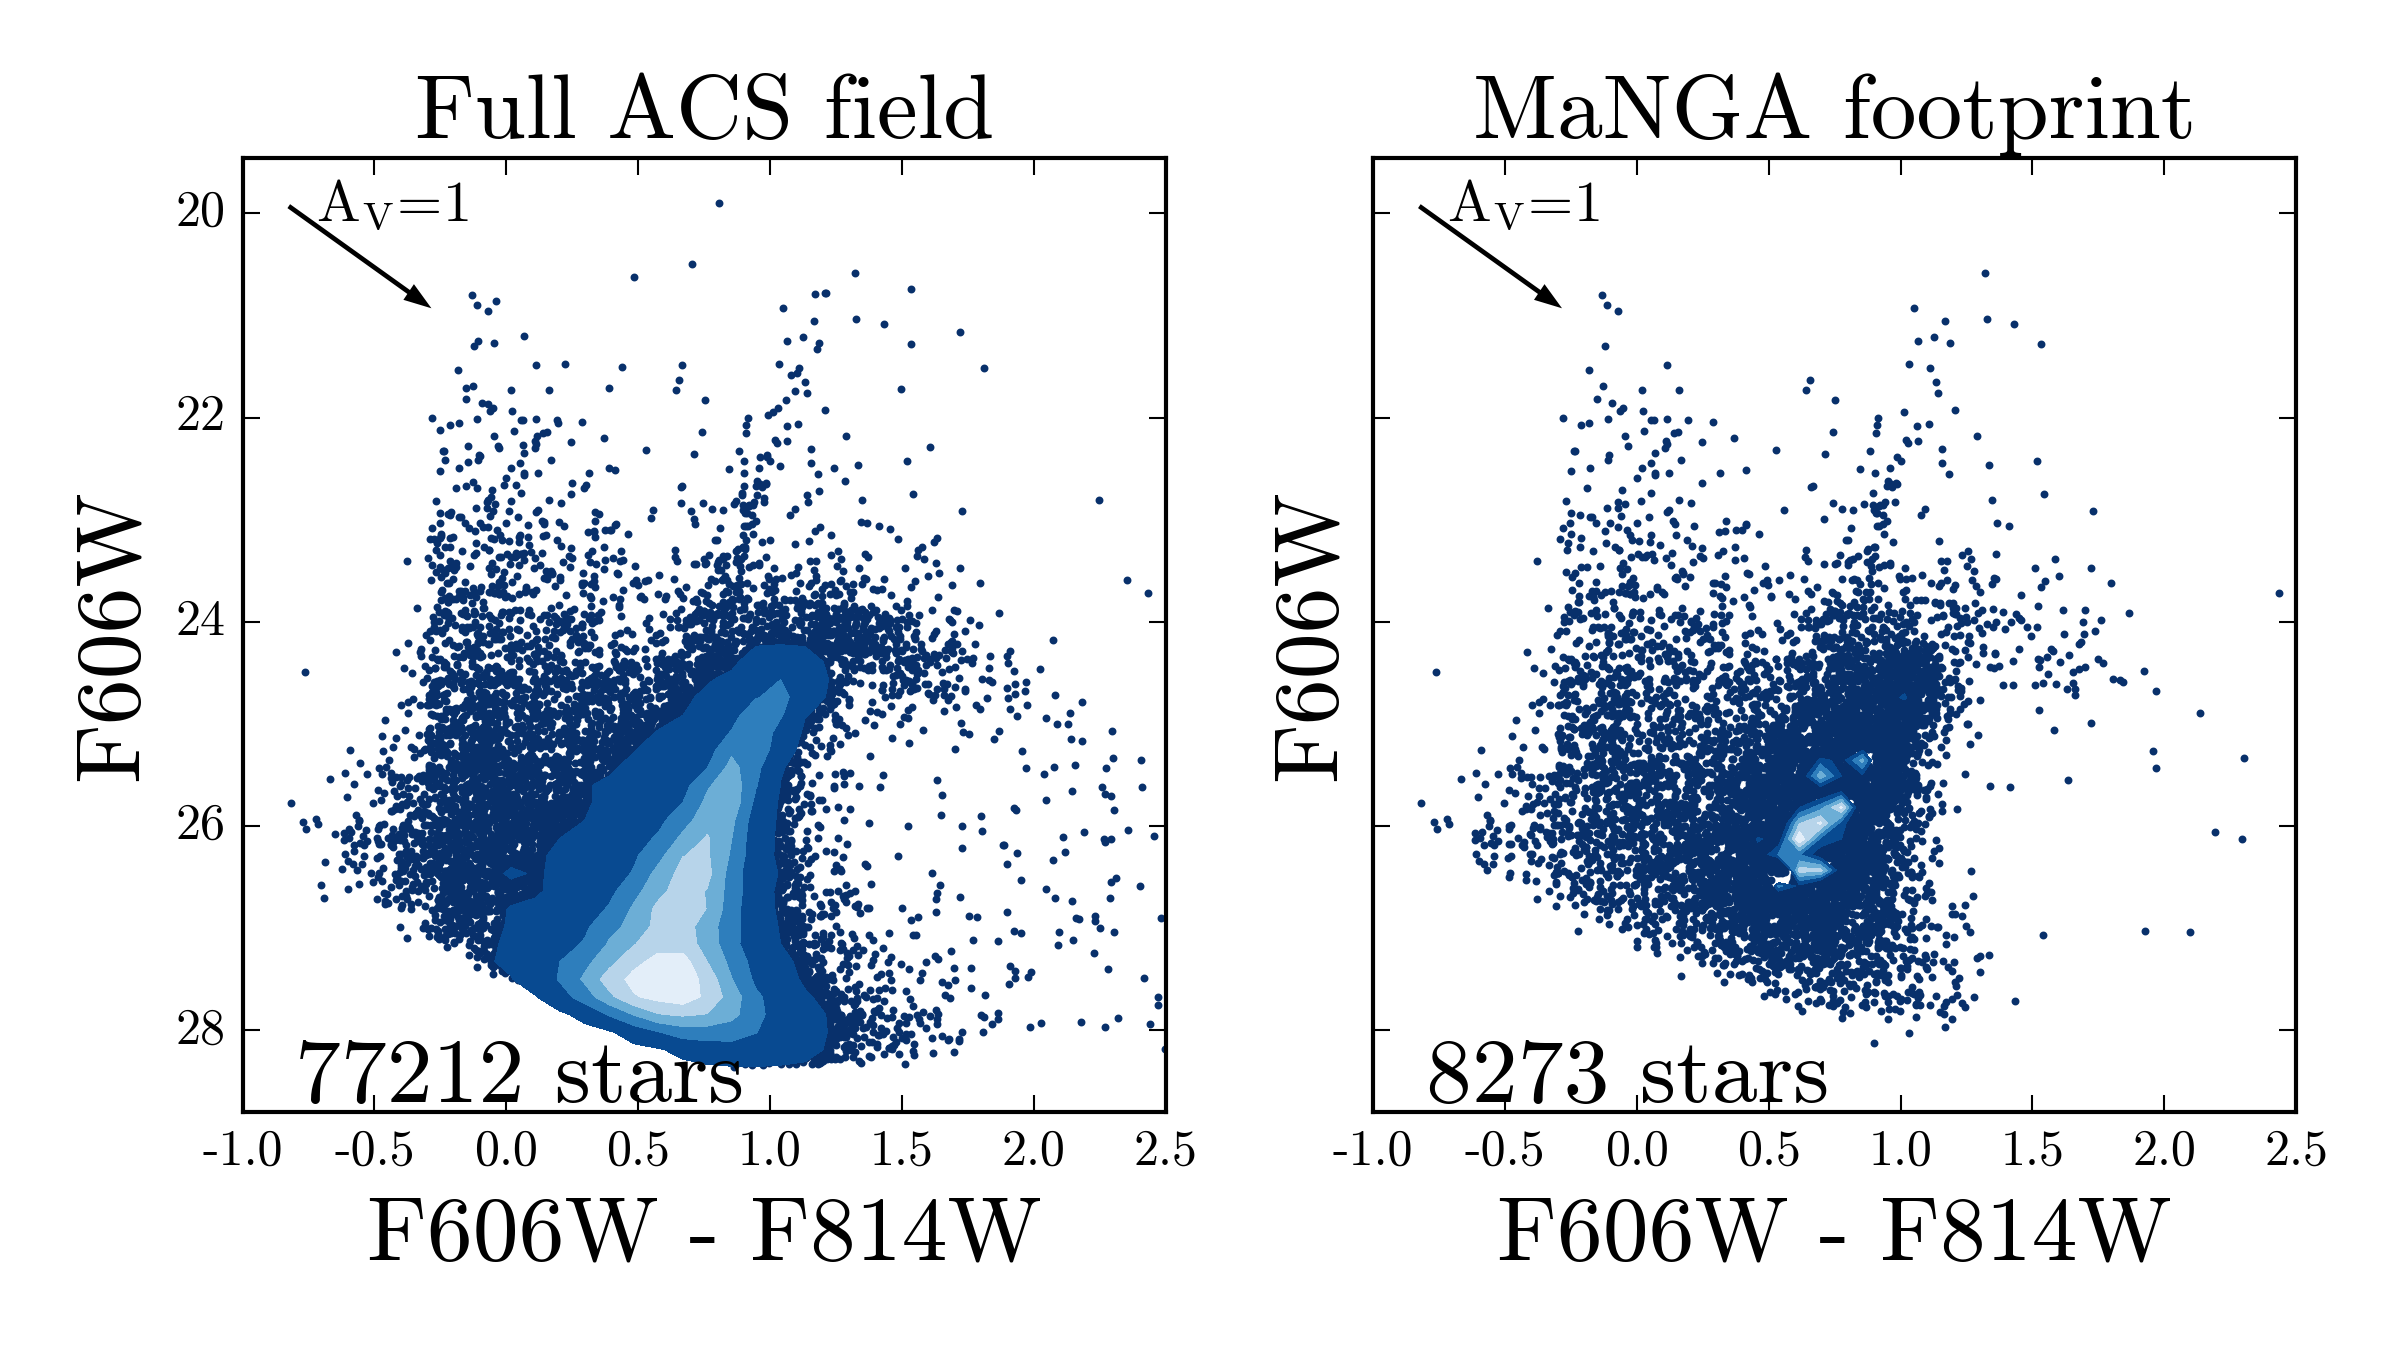
\includegraphics[width=\linewidth]{figs/f2.png}
    \caption{\emph{Left:} The CMD for the full ACS field of view, which includes ${\sim}77,000$ stars. \emph{Right: } The CMD of stars extracted from the region mapped to the MaNGA observations, which includes ${\sim}9,000$ stars. The photometry in the aperture-matched region is significantly shallower than the photometry from the full field, due to higher crowding in the central region of the galaxy.}
    \label{fig:cmd}
  \end{center}
\end{figure*}
%-------------------------------------------------------

\subsubsection{Artificial Star tests}

To characterize the photometric completeness and account for observational errors that result from crowding, we preform extensive artificial star tests (ASTs). In these tests, we insert fake stars into each image and rerun the photometry as before. We test for the recovery of these fake stars, and measure the difference between the input and recovered magnitude if the star was detected. The ASTs are used to construct a noise model that accounts for completeness, photometric uncertainties, and color or magnitude biases.

The region covered by the MaNGA observations is significantly more crowded than the full ACS field-of-view. When running MATCH on the CMD from the aperture-matched region, we used a sample of fake stars representative of those found in the crowded central region. In total, we inserted $565,659$ artificial stars individually into the full ACS image. The aperture-matched region contains the results of $65,318$ ASTs.

We show the results from the aperture-matched ASTs in Fig.~\ref{fig:comp}, showing the photometric completeness as a function of magnitude for the F606W filter (left) and the F814W filter (right). In both panels, the red line represents the magnitude at which 50\% of the inserted fake stars are recovered.

%-------------------------------------------------------
% Figure 3: AST 50% completeness
%-------------------------------------------------------
\begin{figure}
  \begin{center}
    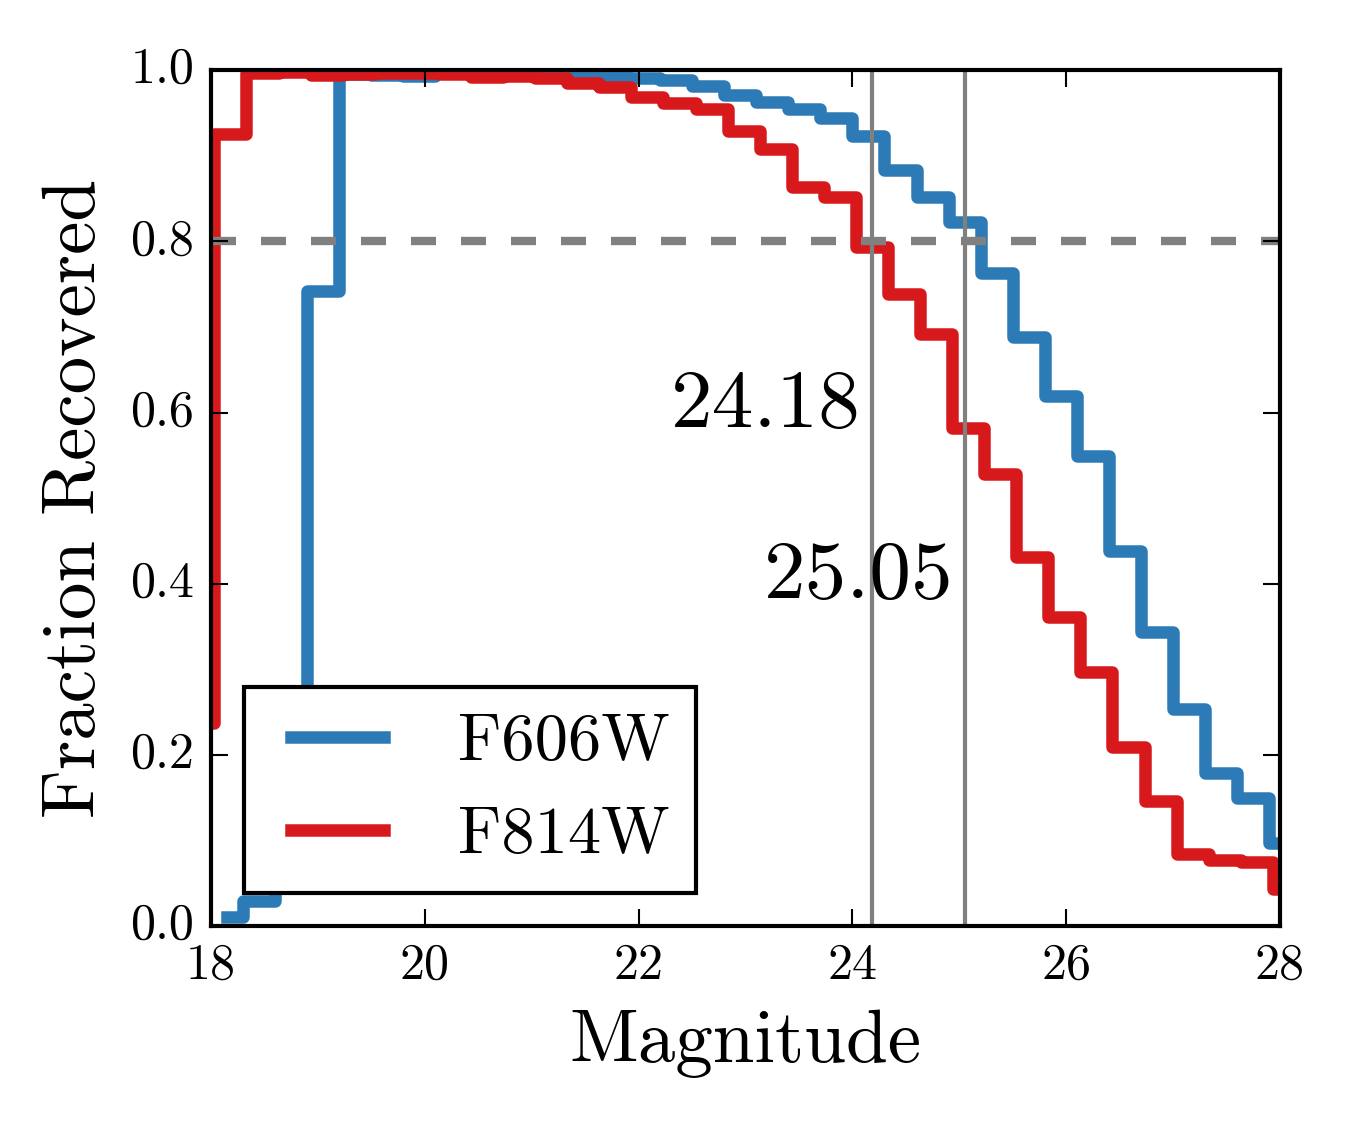
\includegraphics[width=\linewidth]{figs/f3.png}
    \caption{The 50\% completeness limit for the F606W filter (blue) and the F814W filter (red), computed using fake stars representative of the spatial region mapped to the location of the MaNGA observations.}
    \label{fig:comp}
  \end{center}
\end{figure}
%-------------------------------------------------------


\section{Methods}\label{sec:methods}

Broadly, the procedure for the aperture matched comparison is as follows: We extract HST stellar photometry from the area matched to the MaNGA observation, and fit the CMD of those stars using MATCH \citep{Dolphin+2002} to derive the history of star formation, the chemical evolution history, total stellar mass, and the total and differential extinction. We use the CMD-inferred properties as inputs to the SPS code FSPS \citep{Conroy+2009} to produce a model spectrum, which we compare to the total integrated spectrum observed with MaNGA. Additionally, we use the spectral fitting code Prospector (Johnson et al., \emph{in prep}) to fit the total integrated spectrum from MaNGA, to compare the SFH determinations from CMD and integrated light techniques. We detail each of these steps below.

\subsection{MATCH input parameters}\label{sec:methods:match}

We measure the SFH of NGC 4163 using the maximum likelihood CMD fitting routine, MATCH \citep{Dolphin+2002}. For a set of input parameters (e.g., IMF slope, binary fraction, age bin width, etc.) MATCH constructs synthetic CMDs from SSPs and linearly combines them with a model foreground CMD to form a composite model CMD with a complex SFH. The CMD is convolved with the noise model generated from the ASTs. The model CMD is compared with the observed CMD using a Poisson likelihood statistic. The process is repeated for various weights on the SSPs until the likelihood function is maximized. The synthetic CMD that best matches the observed CMD is deemed to have the most likely SFH that produced the data. Full details are given in \citet{Dolphin+2002}.

In this work we have adopted the following parameters for the SFH solutions, summarized in Table~\ref{tab2}. As discussed in \S\ref{sec:data:hst}, we assume a fixed distance modulus of $\dmod = 27.33$. We assume a \citet{Chabrier+2003} IMF, and a binary fraction of 0.35, with the mass of the secondary drawn from a uniform distribution of mass ratios. We use the C3K theoretical spectral library and the MIST stellar evolution models from \citet{Choi+2016, Dotter+2016}, with mass limits from 0.1 to 300\Msun. We used the combination of MIST and C3K so that the same isochrones and stellar library are used to fit the CMD \emph{and} to generate the synthetic spectrum in FSPS. We discuss the use of alternative isochrones and stellar spectral libraries in \ref{sec:discussion}.

\paragraph{SFH specifications}

Due to the shallow photometric depth in the aperture-matched region, we derive the SFHs using only the optical data from the F606W and F814W filters, which provide the deepest CMDs. We designated the faint photometric limit to be equal to the 50\% completeness limit in each filter (see Table~\ref{tab2}) as determined by the artificial star tests run for each galaxy. We discuss the use of more conservative photometric limits (at the 80\% completeness limit) in \ref{sec:discussion}.

We solve for the SFH in 68 time bins covering a range in log time from 6.6 to 10.15 years, spaced by 0.1 dex between 6.6 and 8.7, and by 0.05 dex between 8.7 and 10.15. We are limited by the depth of the data, which does not reach the red clump, and so we constrain the metallicity to only increase with time. We limit the oldest time bins to have [M/H] between -2.5 and -1.0 and the youngest time bin to have [M/H] between -1.0 and 0.0. Within each time bin, however, we permitted a $1\sigma$ metallicity dispersion of 0.15 dex, which provides the flexibility to capture potential metallicity spreads at each age.

\paragraph{Dust}
MATCH allows two free parameters to describe the dust distribution: a foreground extinction, \Av, and a differential extinction, \dAv, which describes the spread in extinction values for the stars in the region. The differential extinction is a step function starting at \Av with a width given by \dAv. As discussed in \S\ref{sec:data:hst}, we assume that the foreground extinction is fixed at \Av$=0.06$. However, we allow \dAv to vary between 0.0 and 1.0.

We use an age-dependent differential extinction model for stars with ages $<100$\Myr, as specified in \citet{Dolphin+2003}. In this model, stars with ages between 100 and 40\Myr have a linearly increasing maximum differential extinction, from \Av(max)$= 0.0$ at 100\Myr to \Av(max)$= 0.5$ mag at 40\Myr. Stars with ages below $40$\Myr have a maximum extinction of 0.5 mag in \Av. This model provides optimal fits to the young stellar populations in a variety of nearby dwarf galaxies \citep[e.g.,][]{Dolphin+2003, Skillman+2003, Weisz+2011}, and is necessary to reproduce the observed integrated blue-optical and ultraviolet light of dwarf galaxies in the Local Volume \citep{Johnson+2013}.

\subsection{Generating model spectrum with FSPS using the CMD-inferred SFH}\label{sec:methods:fsps}

In this section, we describe the process for generating the model spectrum using the CMD-derived SFH. 

For stellar population synthesis, we use the Flexible Stellar Population Synthesis package \citep[\FSPS;][]{Conroy+2009, Conroy+2010} via the Python interface, \pFSPS \citep{pythonFSPSdfm}. We note that the isochrone set, spectral library, and IMF used to construct the model spectrum are identical to those used within MATCH for CMD fitting, to make the most robust comparison.

Specifically, we use the MESA Isochrones \& Stellar Tracks \citep[MIST;][]{Dotter+2016, Choi+2016}, single-star stellar evolutionary models which include the effect of stellar rotation. The evolutionary tracks are computed using the publicly available stellar evolution package Modules for Experiments in Stellar Astrophysics \citep[MESA v7503;][]{Paxton+2011,Paxton+2013, Paxton+2015}. We combine the MIST tracks with a high resolution theoretical spectral library (C3K; Conroy, Kurucz, Cargile, Castelli, \emph{in prep}) based on Kurucz stellar atmosphere and spectral synthesis routines \citep[ATLAS12 and SYNTHE,][]{Kurucz+2005}. For all other SPS parameters, we use the default parameters in \FSPS\footnote{GitHub commit hash \texttt{4e1b3f5}}.

\paragraph{SFH and age-metallicity relation}
To generate our model spectrum, we use three outputs from MATCH: (1) the total stellar mass formed in the area observed, (2) the fraction of the total stellar mass formed within each time interval, and (3) the metallicity of the stars formed in each time interval. We refer to the combination of (1) and (2) as the CMD-based SFH, and (3) as the CMD-based chemical evolution history, or CEH.

We first resample the MATCH SFH and CEH onto the more finely sampled native time resolution of the isochrones, ensuring that the mass integrated over the MATCH time interval is preserved in the resampled SFH. This process implicitly assumes a constant SFH throughout the duration of each time bin. At each time step, we select the SSP with metallicity determined by the CEH, and generate a spectrum. This process leaves us with an array of SSP spectra at each age.

We redden each model spectrum using both the foreground extinction \Av, and the differential extinction \dAv returned by MATCH. We use the same age-dependent differential extinction model used during the CMD-fitting process, with the best-fit value of \dAv=0.4 to scale the maximum differential extinction.

We sum the array of SSP spectra, weighting each spectrum by the fraction of mass formed at that age, as determined from the SFH. The result is a single spectrum, reflecting the mass-weighted ages and chemical compositions from the CMD-derived SFH and CEH.

To compare the synthesized spectrum with the total observed spectrum from MaNGA, we use the distance modulus assumed in \S\ref{sec:methods:match} to scale the absolute flux level of the model spectrum, which we convert to $10^{-17}$erg/s/cm$^2$/\ang, the units of the observed spectrum.

\paragraph{Spectral Resolution}

The C3K library has R=10,000 between 1500\ang and 10,000\ang. The MaNGA observations typically have spectral resolution $R\sim2000$, so we smooth the model spectrum with a wavelength dependent line-spread function. We use the wavelength array, $\lambda_{\mathrm{MaNGA}}$, from the MaNGA datacube (de-redshifted using the redshift from the Data Analysis Pipeline $z=0.000547$ XXX check this number) and the associated spectral resolution array, $R_{\mathrm{MaNGA}}$ (i.e., $\lambda$/d$\lambda$) which provides the median spectral resolution as a function of wavelength for the fibers in the IFU. To compute $\sigma_{\mathrm{MaNGA}}$, the dispersion in \ang, we divide the wavelength array, $\lambda_{\mathrm{MaNGA}}$, by the spectral resolution array, $R_{\mathrm{MaNGA}}$. We then divide $\sigma_{\mathrm{MaNGA}}$ by 2.355 to convert to FWHM, giving the wavelength-dependent line-spread function {\tt lsf}$_{\mathrm{MaNGA}}$. We interpolate {\tt lsf}$_{\mathrm{MaNGA}}$ onto the model wavelength array, and then smooth the model spectrum using {\tt lsf}$_{\mathrm{MaNGA}}$ with a FFT convolution. We note that this process does not correct for the template resolution of the spectral library. However, this should only present an issue if we are interested in making detailed kinematic comparisons. We thus choose to omit the correction. \textbf{XXX BDJ: is this true?}
 
\paragraph{Nebular Emission}

We generate two model spectra: one that includes nebular line and continuum emission, and one that does not. For the spectrum that includes nebular emission, we use the \Cloudy nebular model implemented within \FSPS, \CloudyFSPS \citep{cloudyFSPSv1}, which scales the nebular emission with the ionizing photon flux from the stellar spectrum. The full details of the nebular model can be found in \citet{Byler+2017}.

We emphasize that MATCH is not sensitive to stellar populations with ages below 4\Myr (\textbf{XXX: because? sampling of upper IMF?}), and thus is unable to provide any constraints on the nebular emission properties, and our assessment of the nebular emission is only qualitative. The gas phase metallicity is scaled to match the present-day stellar metallicity, inferred from the CMD. We assume a modest value for the ionization parameter, \logU, (\logUeq{-4}), since the emission morphology is quite diffuse, and several low ionization lines are observed (e.g., \sii).

\subsection{Spectral fitting on the total MaNGA spectrum with \emph{Prospector}}\label{sec:methods:pros}

Description of Prospector and input parameters for spectral fitting from Grace.

\section{Results}\label{sec:results}

\subsection{MATCH results}\label{sec:results:match}

\paragraph{The best fit model CMD}

In Fig.~\ref{fig:matchCMD} we show the results of the CMD-fitting process for NGC 4163. We show Hess diagrams (a 2D density plot of the CMD) for the observed data (a), the best fit model (b), the total residual difference between model and data (c) and the residual significance (d). Overall, we find that the model reproduces the observed CMD reasonably well. The best fit model contains an RGB, SGB, and MS that are well matched to the observations in terms of density of stars, luminosities/colors, and width of features.

Examining the residual significance CMD, i.e., the difference between the data and the model weighted by the variance (the lower right panel of Fig.~\ref{fig:matchCMD}), we can see that the fit is not perfect. In particular, the area between the young stars on the main sequence and the blue helium-burning stars (which bracket F606W-F814W$\,{\sim}\,0$) appears to be too cleanly separated in the model. This discrepancy could indicate that the young stars in the observed CMD are affected by more differential extinction than accounted for in MATCH. However, there are few coherent structures visible in the residual significance Hess diagram (panel (d) of Fig.~\ref{fig:matchCMD}), and even the most discrepant regions are fit within $\pm 5\sigma$, as indicated by the black or white pixels. As such, the perception of difference is not obviously statistically significant.

The best-fit maximum differential extinction for the young populations is $\dAv = 0.4$ mag, which is typical of other local star forming dwarf galaxies \citep{Weisz+2011}. However, the aperture-matched region shows clear spatial variations in the young stellar populations (e.g., Fig.~\ref{fig:FOV}), and it is likely that there are also significant spatial variations in differential extinction. Regions where the differential extinction differs significantly from the best-fit value introduce additional uncertainties associated with the youngest time bin fit by MATCH. We further discuss the sensitivity to variations in differential extinction in \S\ref{sec:discussion:dav}.

%-------------------------------------------------------
% Figure 4: Hess diagrams and residuals
%-------------------------------------------------------
\begin{figure}
  \begin{center}
    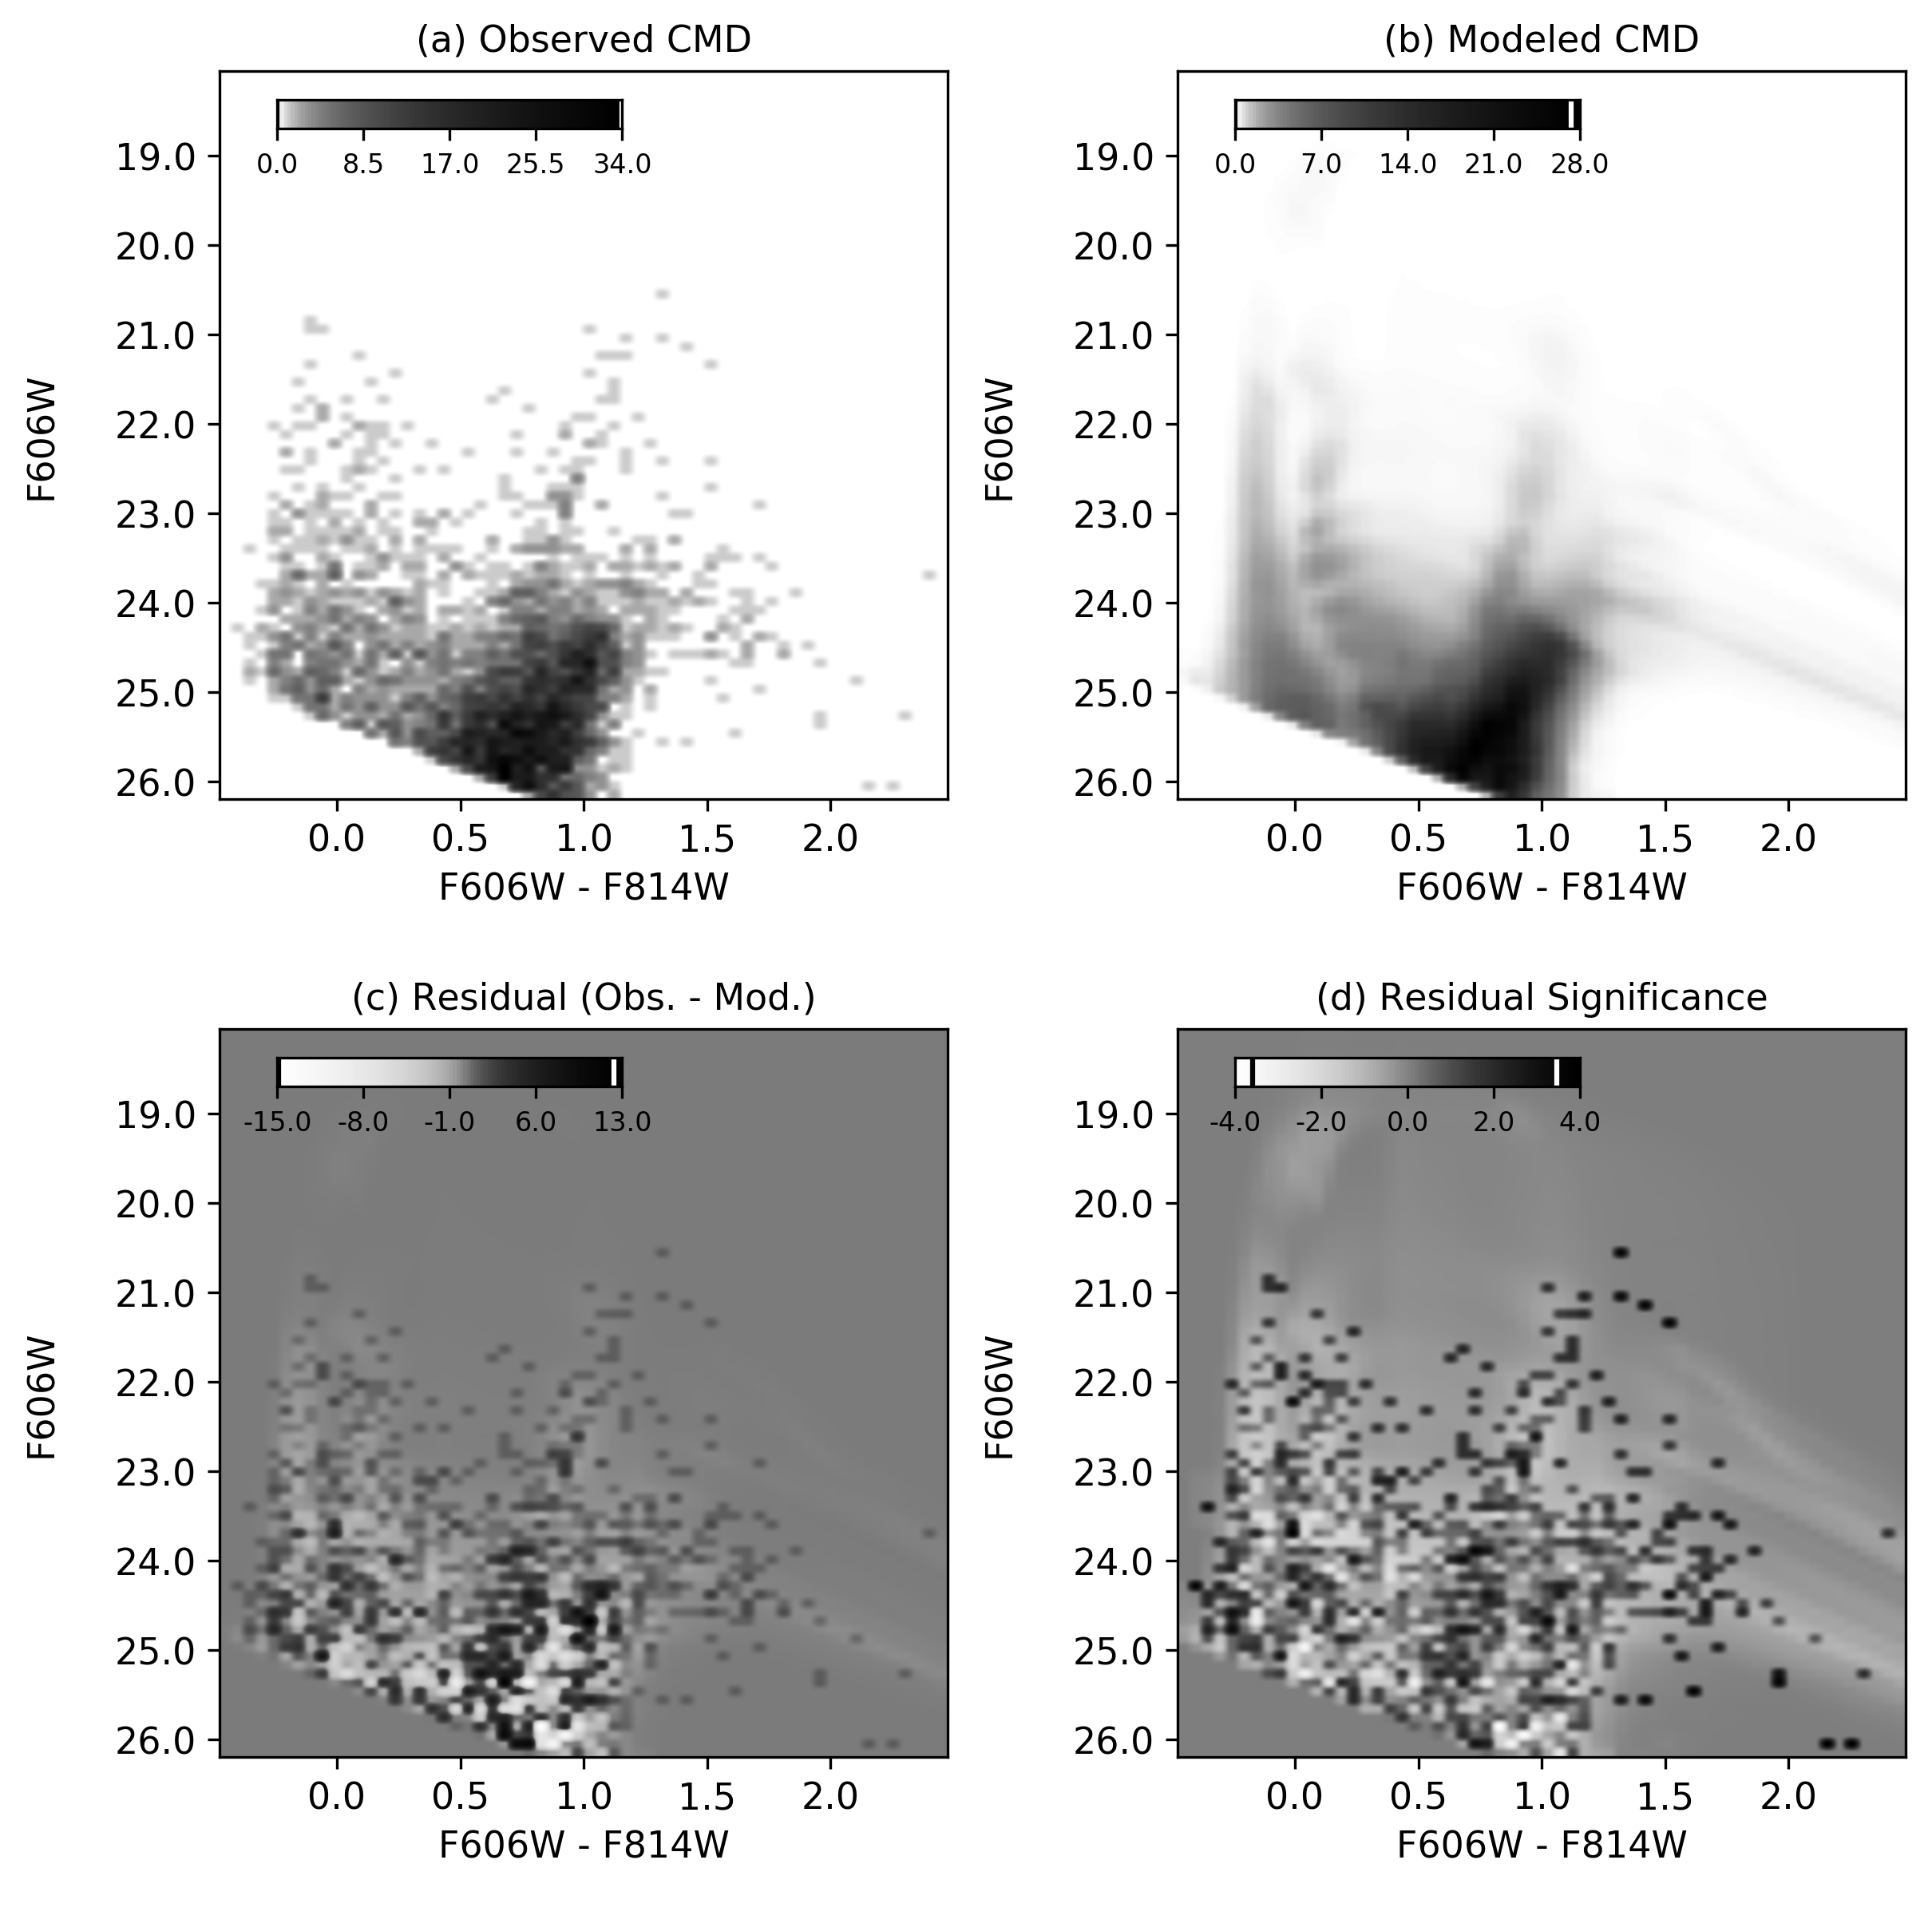
\includegraphics[width=\linewidth]{figs/figMATCH.png}
    \caption{(a) The observed Hess diagram; (b) the best fit model Hess diagram; (c) residual Hess diagram; (d) residual significance Hess diagram. i.e., the difference between model and data weighted by the variance. In panels (a), (b) and (c), the greyscale reflects the number of stars. In panel (d), the greyscale reflects the significance of each pixel in the residual relative to the standard deviation of a Poisson distribution. Overall, the model reproduces the observed Hess diagram reasonably well, demonstrated in the lack of coherent structure in panel (d). \textbf{what are the white and black lines in the residual significance colorbar?}}
    \label{fig:matchCMD}
  \end{center}
\end{figure}
%-------------------------------------------------------
\paragraph{The best-fit star formation history}

In Fig.~\ref{fig:matchSFH}, we show the best fit SFHs for NGC 4163. In the left panel, we show the best fit absolute SFH, or the SFR as a function of time. In the right panel, we show the cumulative SFH, or the fraction of total stellar mass formed prior to or during a given time bin. In both panels, the results for the aperture-matched CMD are shown in black and the results for the full-field CMD are shown in orange (\textbf{XXX not yet}). The error bars and error envelopes represent the 16$^{\mathrm{th}}$ and 84$^{\mathrm{th}}$ percentile for the distribution of SFHs computed via the Monte Carlo process described in \S\ref{sec:methods:match} (\textbf{XXX not yet}).

The global SFH (as measured from the full-field photometry) and the central, aperture-matched region show similar overall behavior, with a substantial old stellar population (${\sim}50$\% of the total mass) underlying more recent star formation. There is a decline in SFR over the last 100\Myr, with a burst of SF within the last 10\Myr. The aperture-matched region shows a larger fraction of total mass formed in the recent burst of SF, which is expected, considering that the MaNGA observations covered the central part of the galaxy, including several OB associations.

%-------------------------------------------------------
% Figure 5: SFH
%-------------------------------------------------------
\begin{figure}
  \begin{center}
    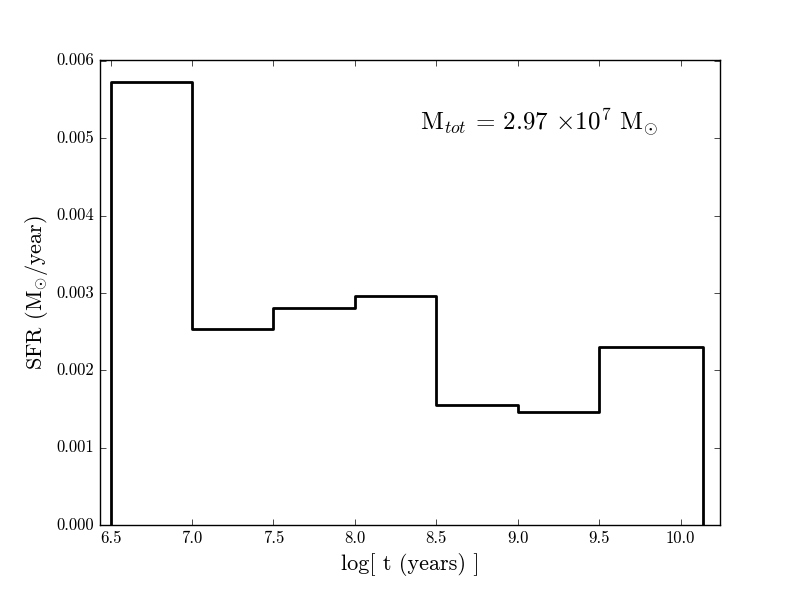
\includegraphics[width=\linewidth]{figs/figSFH.png}
    \caption{The best fit SFH for NGC 4163, including the region matched to the MaNGA observations (black) and the full ACS field of view (orange). The left panel shows the absolute SFH (i.e., the SFR(t)), while the right panel shows the cumulative SFH (i.e., the fraction of total stellar mass formed prior to or during a given time bin. The errorbars (left) and the error envelope (right) represent the 16$^{\mathrm{th}}$ and 84$^{\mathrm{th}}$ percentile for the distribution of SFHs computed via the Monte Carlo process. In the left panel, the grey dashed line represents the lifetime-averaged SFR; in the right panel it shows a slope of unity, i.e., a constant SFR.}
    \label{fig:matchSFH}
  \end{center}
\end{figure}
%-------------------------------------------------------
\paragraph{Other best-fit properties from MATCH}

The full results from the best-fit model from MATCH are given in Table XXX. The present-day metallicity determined from MATCH is [M/H] = -0.6, which is quite close to the metallicity determined by XXX using Be stars.

The aperture-matched region contains $3\times10^7\Msun$ of stars, compared to XXX contained in the full ACS field. As discussed in \S\ref{sec:data:hst}, the shallow photometry in the central region of NGC 4163 and the likelihood of spatial variations in differential extinction and completeness limit the ability of MATCH in determining total stellar mass. \textbf{XXX this seems out of place..the idea was just to state if this was a reasonable total stellar mass.}

\subsection{CMD-inferred model spectrum}

In Fig.~\ref{fig:fullSpec}, we compare the total summed MaNGA spectrum (black) to the model spectrum generated from the CMD-inferred properties (blue) over the full wavelength range observed, $3800-$10,000\ang. The bottom panel shows the percent residual difference between the model and observed spectrum. 

We note that the model spectrum is brighter than the observed spectrum. The mismatch in total flux between model and data is likely due to the shallow, crowded photometry in the region observed by MaNGA (see \S\ref{sec:data:hst} \& \S\ref{sec:methods:match}), which makes it difficult for MATCH to estimate the total stellar mass in the aperture-matched region. We explore other possible explanations for the bulk flux offset in \S\ref{sec:discussion}, including spatial variations in the photometric completeness and differential extinction, and the possibility of missed low-flux spaxels contributing to the total integrated MaNGA spectrum.

In what follows, we continue our comparison between the model and observed spectra, and correct for the flux offset by multiplying the model spectrum by 0.66. After correcting for the flux offset, Fig.~\ref{fig:fullSpec} shows the two spectra have similar overall colors. The model deviates from the observed spectrum at the 5\% level, which is remarkable agreement considering that there has been no fine-tuning of the CMD-inferred properties.

In Figs.~\ref{fig:zoomSpec1}-\ref{fig:zoomSpec3}, we zoom in on key spectral features and compare the CMD-reconstructed spectrum with the observed MaNGA spectrum. As stated in \S\ref{sec:data:hst}, the CMD-fitting process is not-sensitive to stars below 4\Myr, and we keep our discussion of the model-predicted emission lines qualitative.

Fig.~\ref{fig:zoomSpec1} displays the spectrum between 4900\ang and 5400\ang. This region of the spectrum covers several magnesium and iron absorption features that are known to correlate with metallicity. After accounting for the bulk flux offset, the absorption lines are well-matched by the model spectrum, with residual errors of order a few percent. Fig.~\ref{fig:zoomSpec1} also covers two nebular emission lines, \oiii$\lambda$\,4959 and \oiii$\lambda$\,5007. These emission lines are far too strong in the model spectrum, which is not unexpected, since the nebular model assumes 100\% of the ionizing photons are converted into nebular emission, unlikely in this diffuse, porous region.

Fig.~\ref{fig:zoomSpec2} covers 8300\ang to 9000\ang, and includes the calcium triplet. The model does a fairly good job at reproducing the MaNGA spectrum, with residuals of order 5\%. The agreement between model and data is encouraging, because the calcium triplet is a well-known metallicity diagnostic, highlighting the consistency between CMD-derived metallicities and integrated light techniques.

We show the spectrum from 6200\ang to 6800\ang in Fig.~\ref{fig:zoomSpec3}, which covers several nebular emission lines, including \nii$\lambda$\,6548,6584, \ha, and \sii$\lambda$\,6719, 6731. We note that the \sii emission is quite strong in the observed MaNGA spectrum, but very weak in the model. These low ionization features can be associated with diffuse emission (XXX cite kai).

%-------------------------------------------------------
% Figure A: Spectrum [3800-8800]
%-------------------------------------------------------
\begin{figure*}
  \begin{center}
    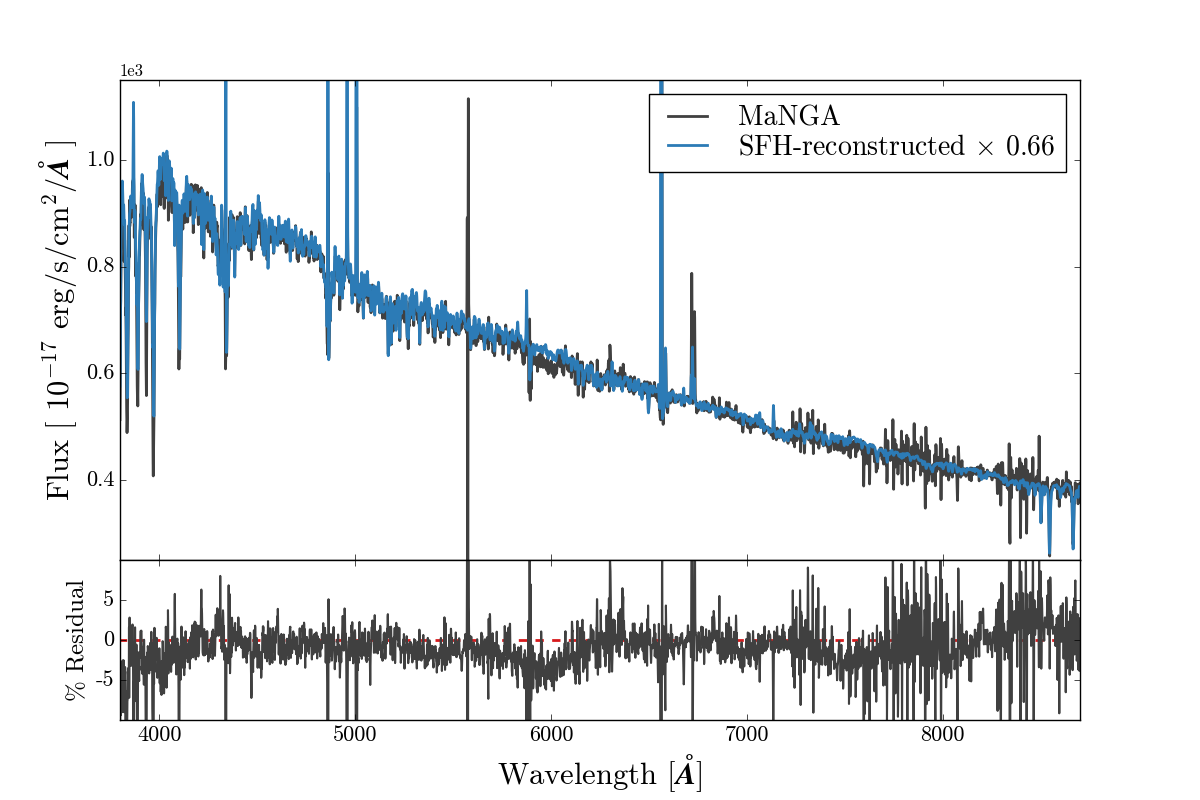
\includegraphics[width=\linewidth]{figs/figA.png}
    \caption{The total summed MaNGA spectrum (black), from 3800 to 8800\ang, compared with the model spectrum synthesized from the CMD-inferred SFH (blue). The bottom panel shows the percent residual error between the observed spectrum and the synthetic spectrum. There is good overall agreement between the data and model spectra, with deviations less than 5\% over the full wavelength range considered. However, we note that the synthesized spectrum has been scaled down by almost 70\% to match the observed flux level, likely a repercussion of the shallow photometry.}
    \label{fig:fullSpec}
  \end{center}
\end{figure*}
%-------------------------------------------------------

%-------------------------------------------------------
% Figure B: Spectrum [4900-5400]
%-------------------------------------------------------
\begin{figure*}
  \begin{center}
    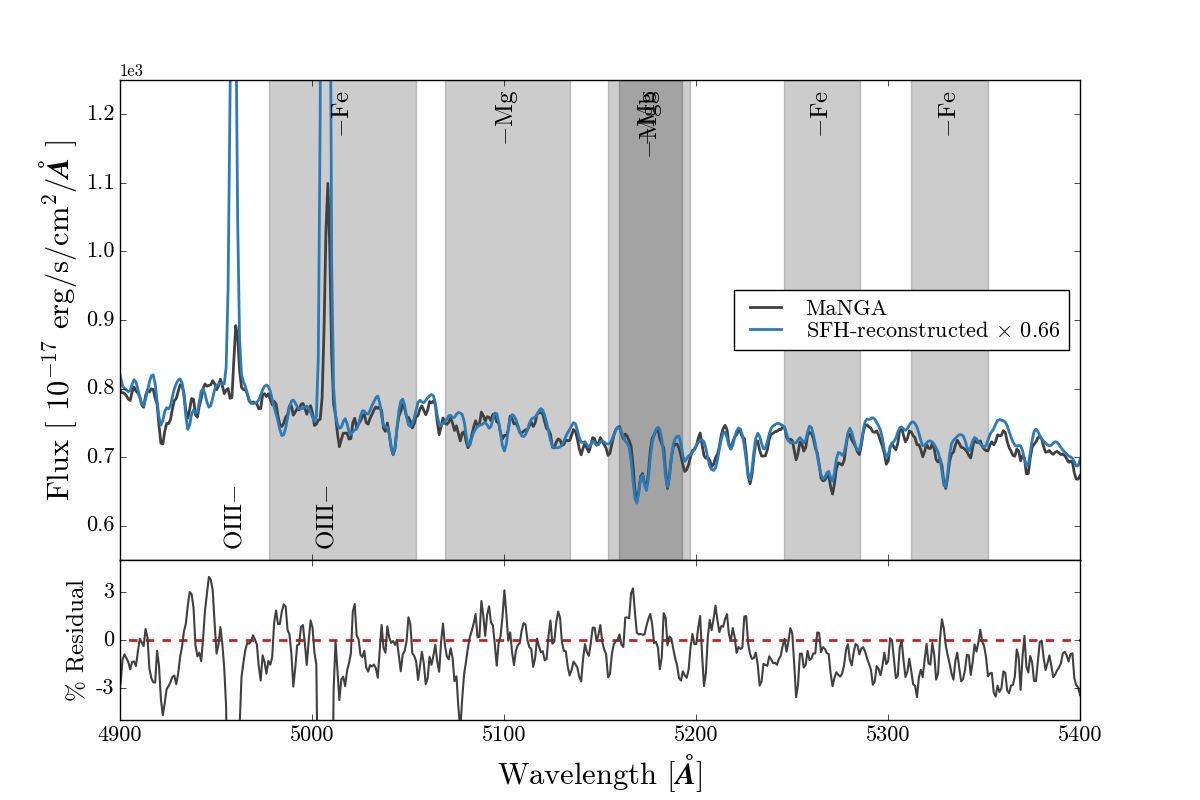
\includegraphics[width=\linewidth]{figs/figB.png}
    \caption{The total summed MaNGA spectrum (black) compared to the model spectrum synthesized from the CMD-based SFH (blue). The percent residual is shown in the bottom panel, with 0\% residuals shown with a red dashed line. The spectrum from 4900 to 5400\ang covers two nebular emission lines (\oiii$\lambda$\,4959 and \oiii$\lambda$\,5007) and magnesium and iron absorption features. The strength of the Mg lines are often used as a stellar metallicity anchor, and it is encouraging that the synthesized spectrum agrees well with the observed spectrum here, despite the overall flux offset.}
    \label{fig:zoomSpec1}
  \end{center}
\end{figure*}
%-------------------------------------------------------

%-------------------------------------------------------
% Figure C: Spectrum [4900-5400]
%-------------------------------------------------------
\begin{figure*}
  \begin{center}
    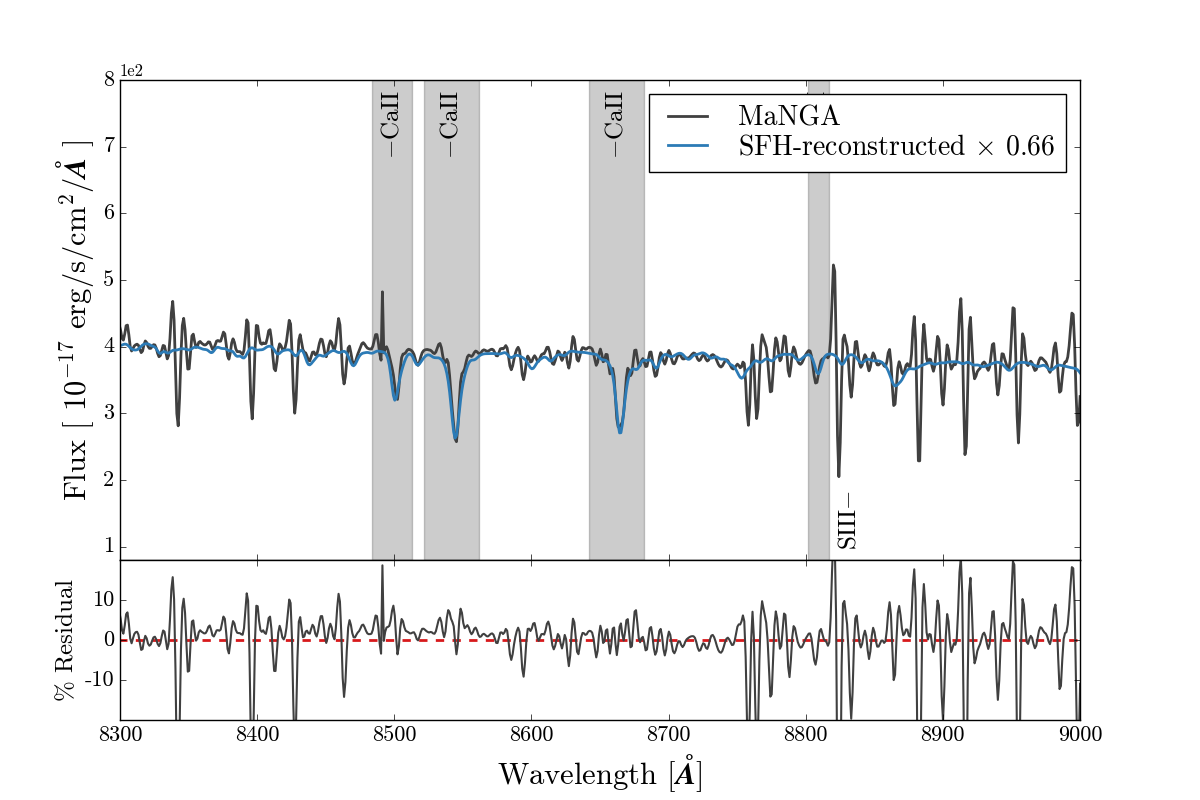
\includegraphics[width=\linewidth]{figs/figC.png}
    \caption{The total summed MaNGA spectrum (black) compared to the model spectrum synthesized from the CMD-based SFH (blue). The percent residual is shown in the bottom panel, with 0\% residuals shown with a red dashed line. The spectrum from 8300 to 9000\ang covers the calcium triplet, which is a frequently used metallicity diagnostic. The synthesized spectrum agrees well with the observed spectrum here, highlighting the consistency between the CMD-inferred metallicity and integrated light techniques.}
    \label{fig:zoomSpec2}
  \end{center}
\end{figure*}
%-------------------------------------------------------

%-------------------------------------------------------
% Figure D: Spectrum [6200-6800]
%-------------------------------------------------------
\begin{figure*}
  \begin{center}
    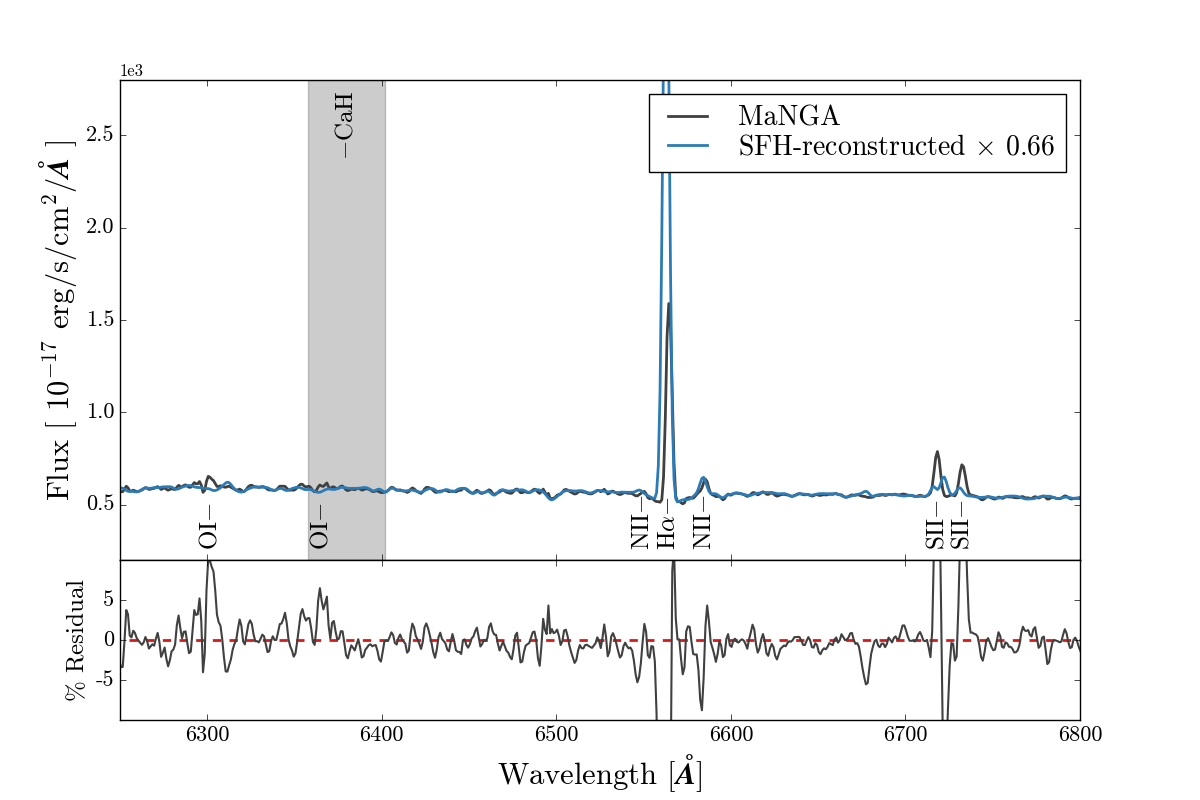
\includegraphics[width=\linewidth]{figs/figD.png}
    \caption{The total summed MaNGA spectrum (black) compared to the model spectrum synthesized from the CMD-based SFH (blue). The percent residual is shown in the bottom panel, with 0\% residuals shown with a red dashed line. The wavelength range from 6200 to 6800\ang covers several nebular emission lines, including \nii$\lambda$\,6548,6584, \ha, and \sii$\lambda$\,6719, 6731. \sii is significantly detected in the observed spectrum, but not predicted in the model spectrum.}
    \label{fig:zoomSpec3}
  \end{center}
\end{figure*}
%-------------------------------------------------------

\subsection{Spectral Fitting with Prospector}\label{sec:results:pros}

Results from Grace here.



\section{Discussion}\label{sec:discussion}

\subsection{Flux offset}\label{sec:discussion:offset}
We have tested to see if the outer spaxels with low-S/N could account for the missing flux, and find that they contribute a few percent of the total flux, at most.


\subsection{Isochrones and Stellar Spectral Library}\label{sec:discussion:iso}

Padova comparison.

\subsection{Spatial variation in differential reddening}\label{sec:discussion:dav}

Due to the non-negligible degree of varying completeness, we may want to measure SFHs on a region-by-region basis, and then combine them as necessary. Initial tests of subregion comparisons have proven to be highly sensitive to spatial variations in differential reddening found in the various star forming knots.

\section{Conclusions}\label{sec:conclusions}

%%%%%%%%%%%%%%%%%%%%%%%%%%%%%%%%%%%%%%%%%%%%%%%%%%%%%%%%%%%%%%%%%%%%%%%%%%%%%%%%
%-------------------------------------------------------
\bibliographystyle{aasjournal}
\bibliography{main}
%-------------------------------------------------------
\end{document}